\section{Content analysis}

\subsection{Homepage contents}

\subsubsection{General consideration}

In addition to what has already been said above, the structure of the 
homepage is very clear and all elements are sufficiently spaced from each 
other. The font size is large, with the purpose of grabbing the user's 
attention. There are graphic elements that make the page interactive and 
enrich it from the point of view of content. In addition, there is an 
animated image with the purpose of illustrating the different possibilities 
of depositing money. It is a good strategy because the user avoids writing 
long text to explain the different deposit possibilities offered by the 
product. Therefore, the cleanliness of the section is maintained, in 
agreement with the others.

\subsubsection{Main menu}

As mentioned previously, the main menu is placed in an ideal position 
(fig. \ref{fig:main-menu}). However, a fundamentally important tool is 
missing: search bar. At first glance, a user would have no way to search 
the contents of the site. This represents a major drawback, which will 
be examined in more detail later.

\subsubsection{Footer}

The website footer is shown in figure \ref{fig:footer}. This section is 
divided into two main parts:
\begin{itemize}
  \item At the top, there are four columns:
  \begin{itemize}
    \item The first column lists all the products developed by the company;

    \item The second column lists a series of pages that illustrate both 
    generic (for example, \textit{Inizia da qui} (\textit{Start here})) and 
    specific (for example, \textit{Comprare Bitcoin} 
    (\textit{Buying Bitcoin})) guides. Redundancy can be found, that is, 
    the \textit{Inizia da qui} and \textit{Young Platform Academy} entries 
    in the first column. In fact, these items point to the same page;

    \item In the third column there are a series of items that point to 
    pages that deal with content strictly related to the company itself. 
    As for the \textit{I nostri prodotti} (\textit{Our products}) entry, 
    I think it would have been more consistent to put it in the first 
    column. This entry redirects to a page that illustrates the various 
    products in a concise and effective way. The 
    \textit{Perché Young Platform} (\textit{Why Young Platform}) entry 
    points to a page that provides reasons to use their products and take 
    advantage of their ecosystem. I believe this page is of some importance 
    in convincing users (both beginners and experts) to use the products. 
    So, I find that the position of this entry is wrong, as the content of 
    that page has some importance;

    \item In the fourth column there are a series of entries that redirect 
    to pages whose contents are very important:
    \begin{itemize}
      \item \textit{Centro di Supporto} (\textit{Support Center}): this item 
      redirects to the same page pointed to by the \textit{Supporto} 
      (\textit{Support}) item of the main menu (fig. \ref{fig:main-menu});

      \item \textit{Commissioni e Prezzi} (\textit{Fees and prices}): 
      redirects to a page that briefly and exhaustively explains the various 
      fees that are applied to the various actions that can be carried out 
      with the various products;

      \item \textit{FAQ *}: these 4 items collect a series of frequently 
      asked questions concerning different topics: \textit{tasse} (taxes), 
      \textit{compravendita} (trading), \textit{commissioni} (fees) and 
      \textit{earning wallet}. I find that this subdivision should not 
      be divided by items but should be divided into a single page. 
      I think it is more useful for the user to have access to all the 
      FAQs on one page. The breakdown of FAQs by topic is useful, but not 
      as implemented on the site. Also, there is no FAQs search tool, 
      which is a disadvantage.
    \end{itemize}
  \end{itemize}

  \item In the lower part, there are the logo and the legal data of the 
  company, a small menu for selecting the language (Italian, English and 
  French), the links to download the applications in the stores and the 
  links of the various social networks.
\end{itemize}

\subsection{Internal pages contents}

As for the internal pages, the obligatory axes are \textit{Who} e 
\textit{What}. The other axes are optional. In particular, the 
\textit{Where} and \textit{Why} axes, while optional, are strongly 
recommended.

\subsubsection{Products page}

The page can be reached at the following address: 
\href{https://youngplatform.com/young-world/}{https://youngplatform.com/young-world/}.

\paragraph{What}

On this page you can clearly understand what is offered. From the title at 
the top of the page it allows you to understand that the various products 
of the company and their differences will be illustrated. In the first 
section (fig. \ref{fig:products-page-1}), the purpose of the page content 
is explained. The other two sections (fig. \ref{fig:products-page-2} and 
\ref{fig:products-page-3}) illustrate the differences between the various 
products, in order to guide the user towards the product best suited to 
his needs.
\begin{figure}[H]
  \centering
  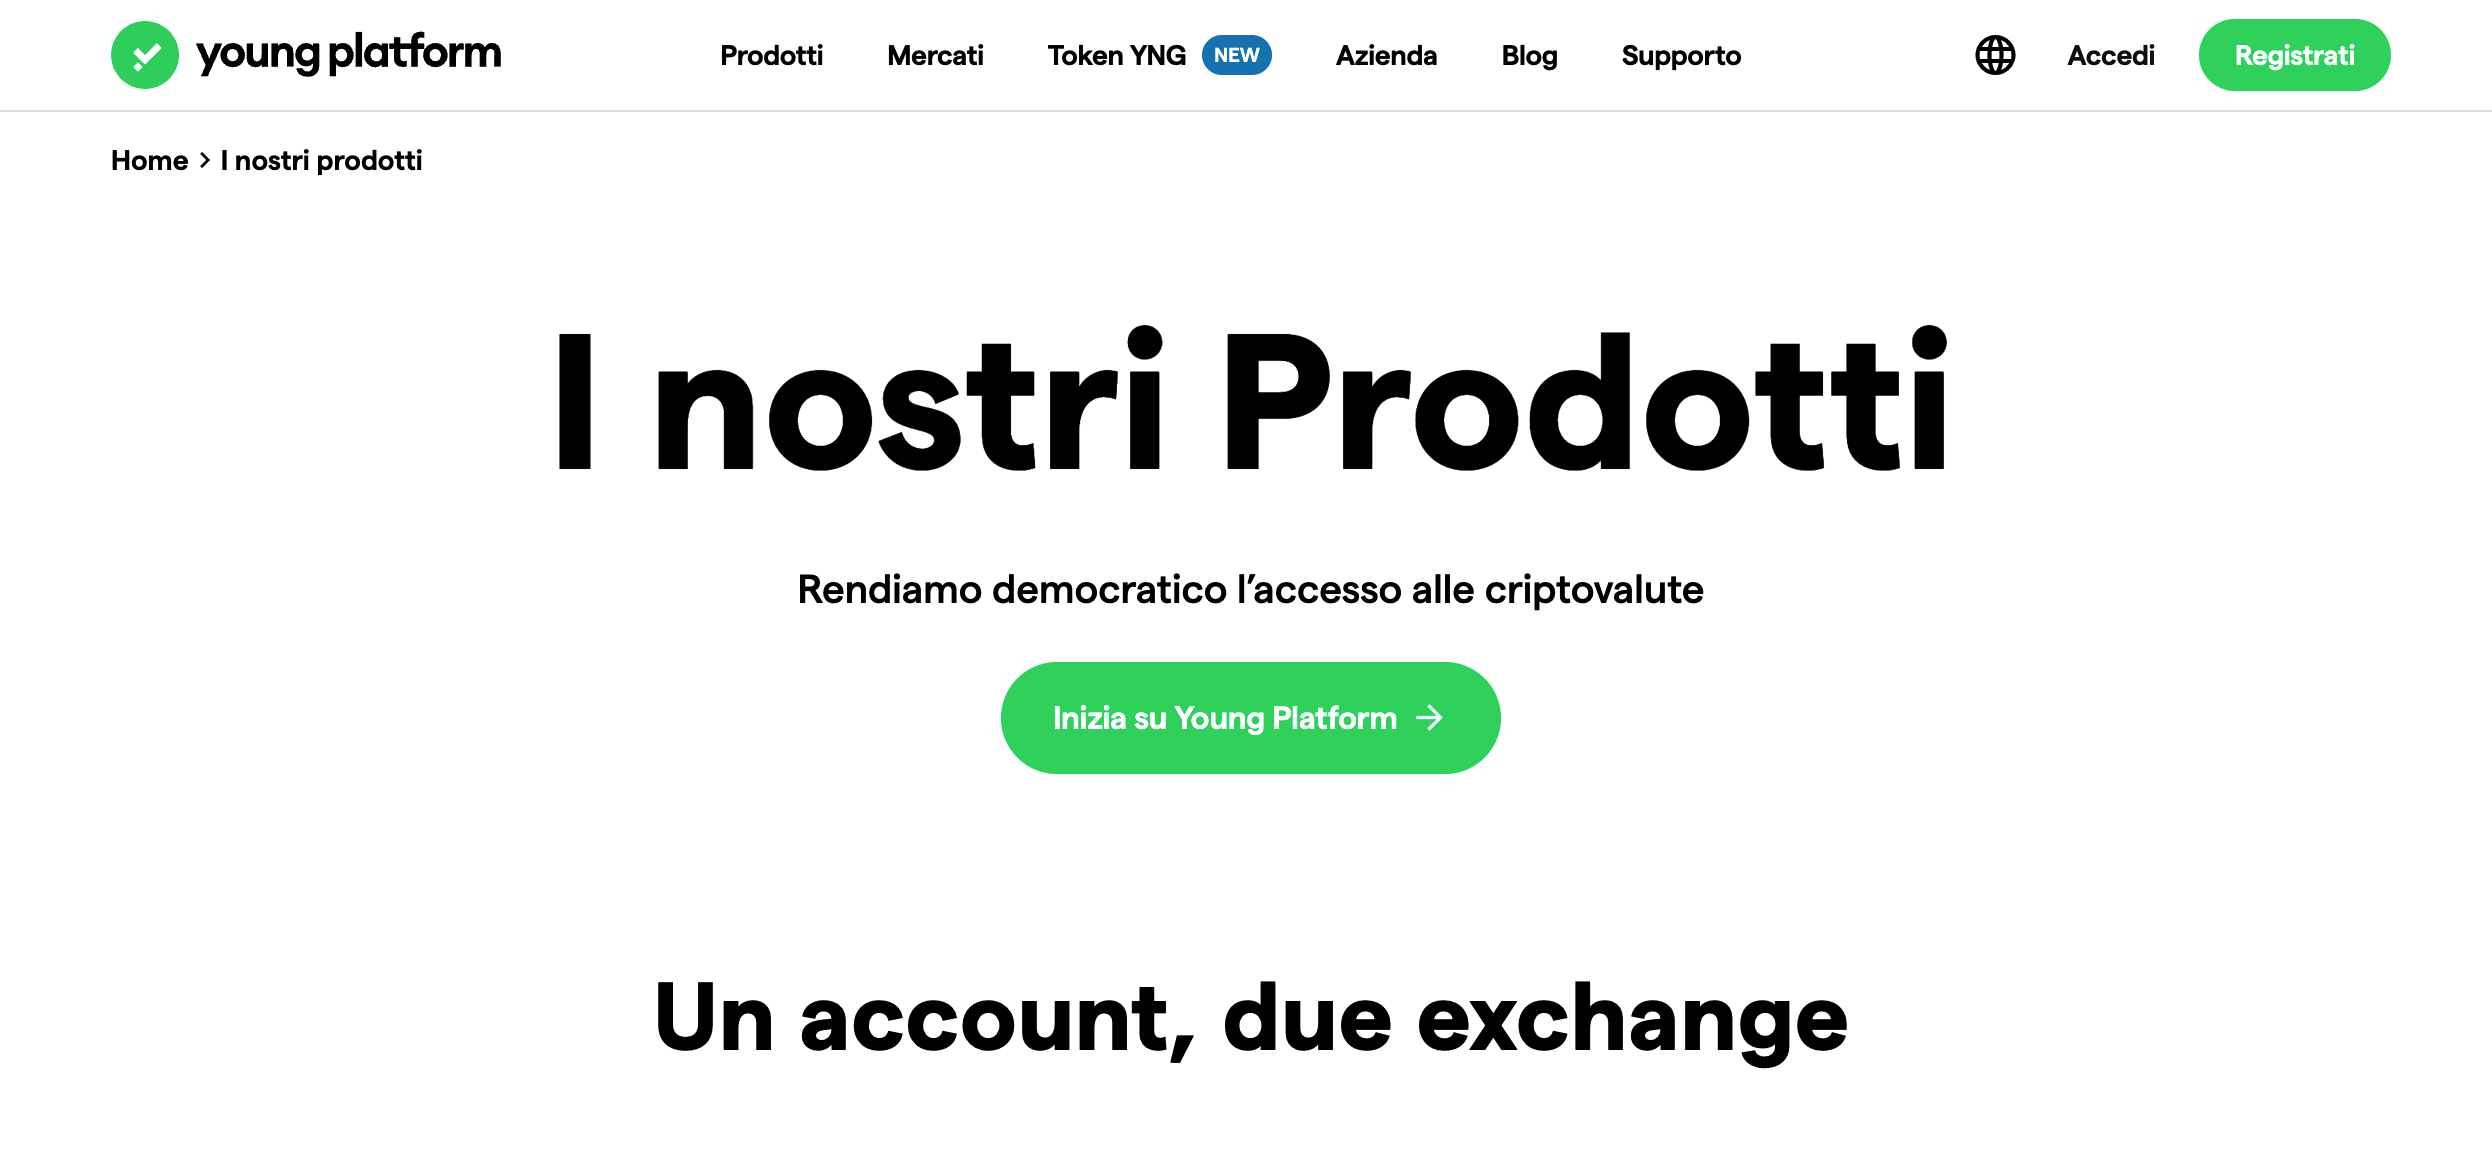
\includegraphics[width=0.70\textwidth]{res/images/internal-pages/products-page/products-page-1.png}
  \caption{First section of the product page.}
  \label{fig:products-page-1}
\end{figure}

\begin{figure}[H]
  \centering
  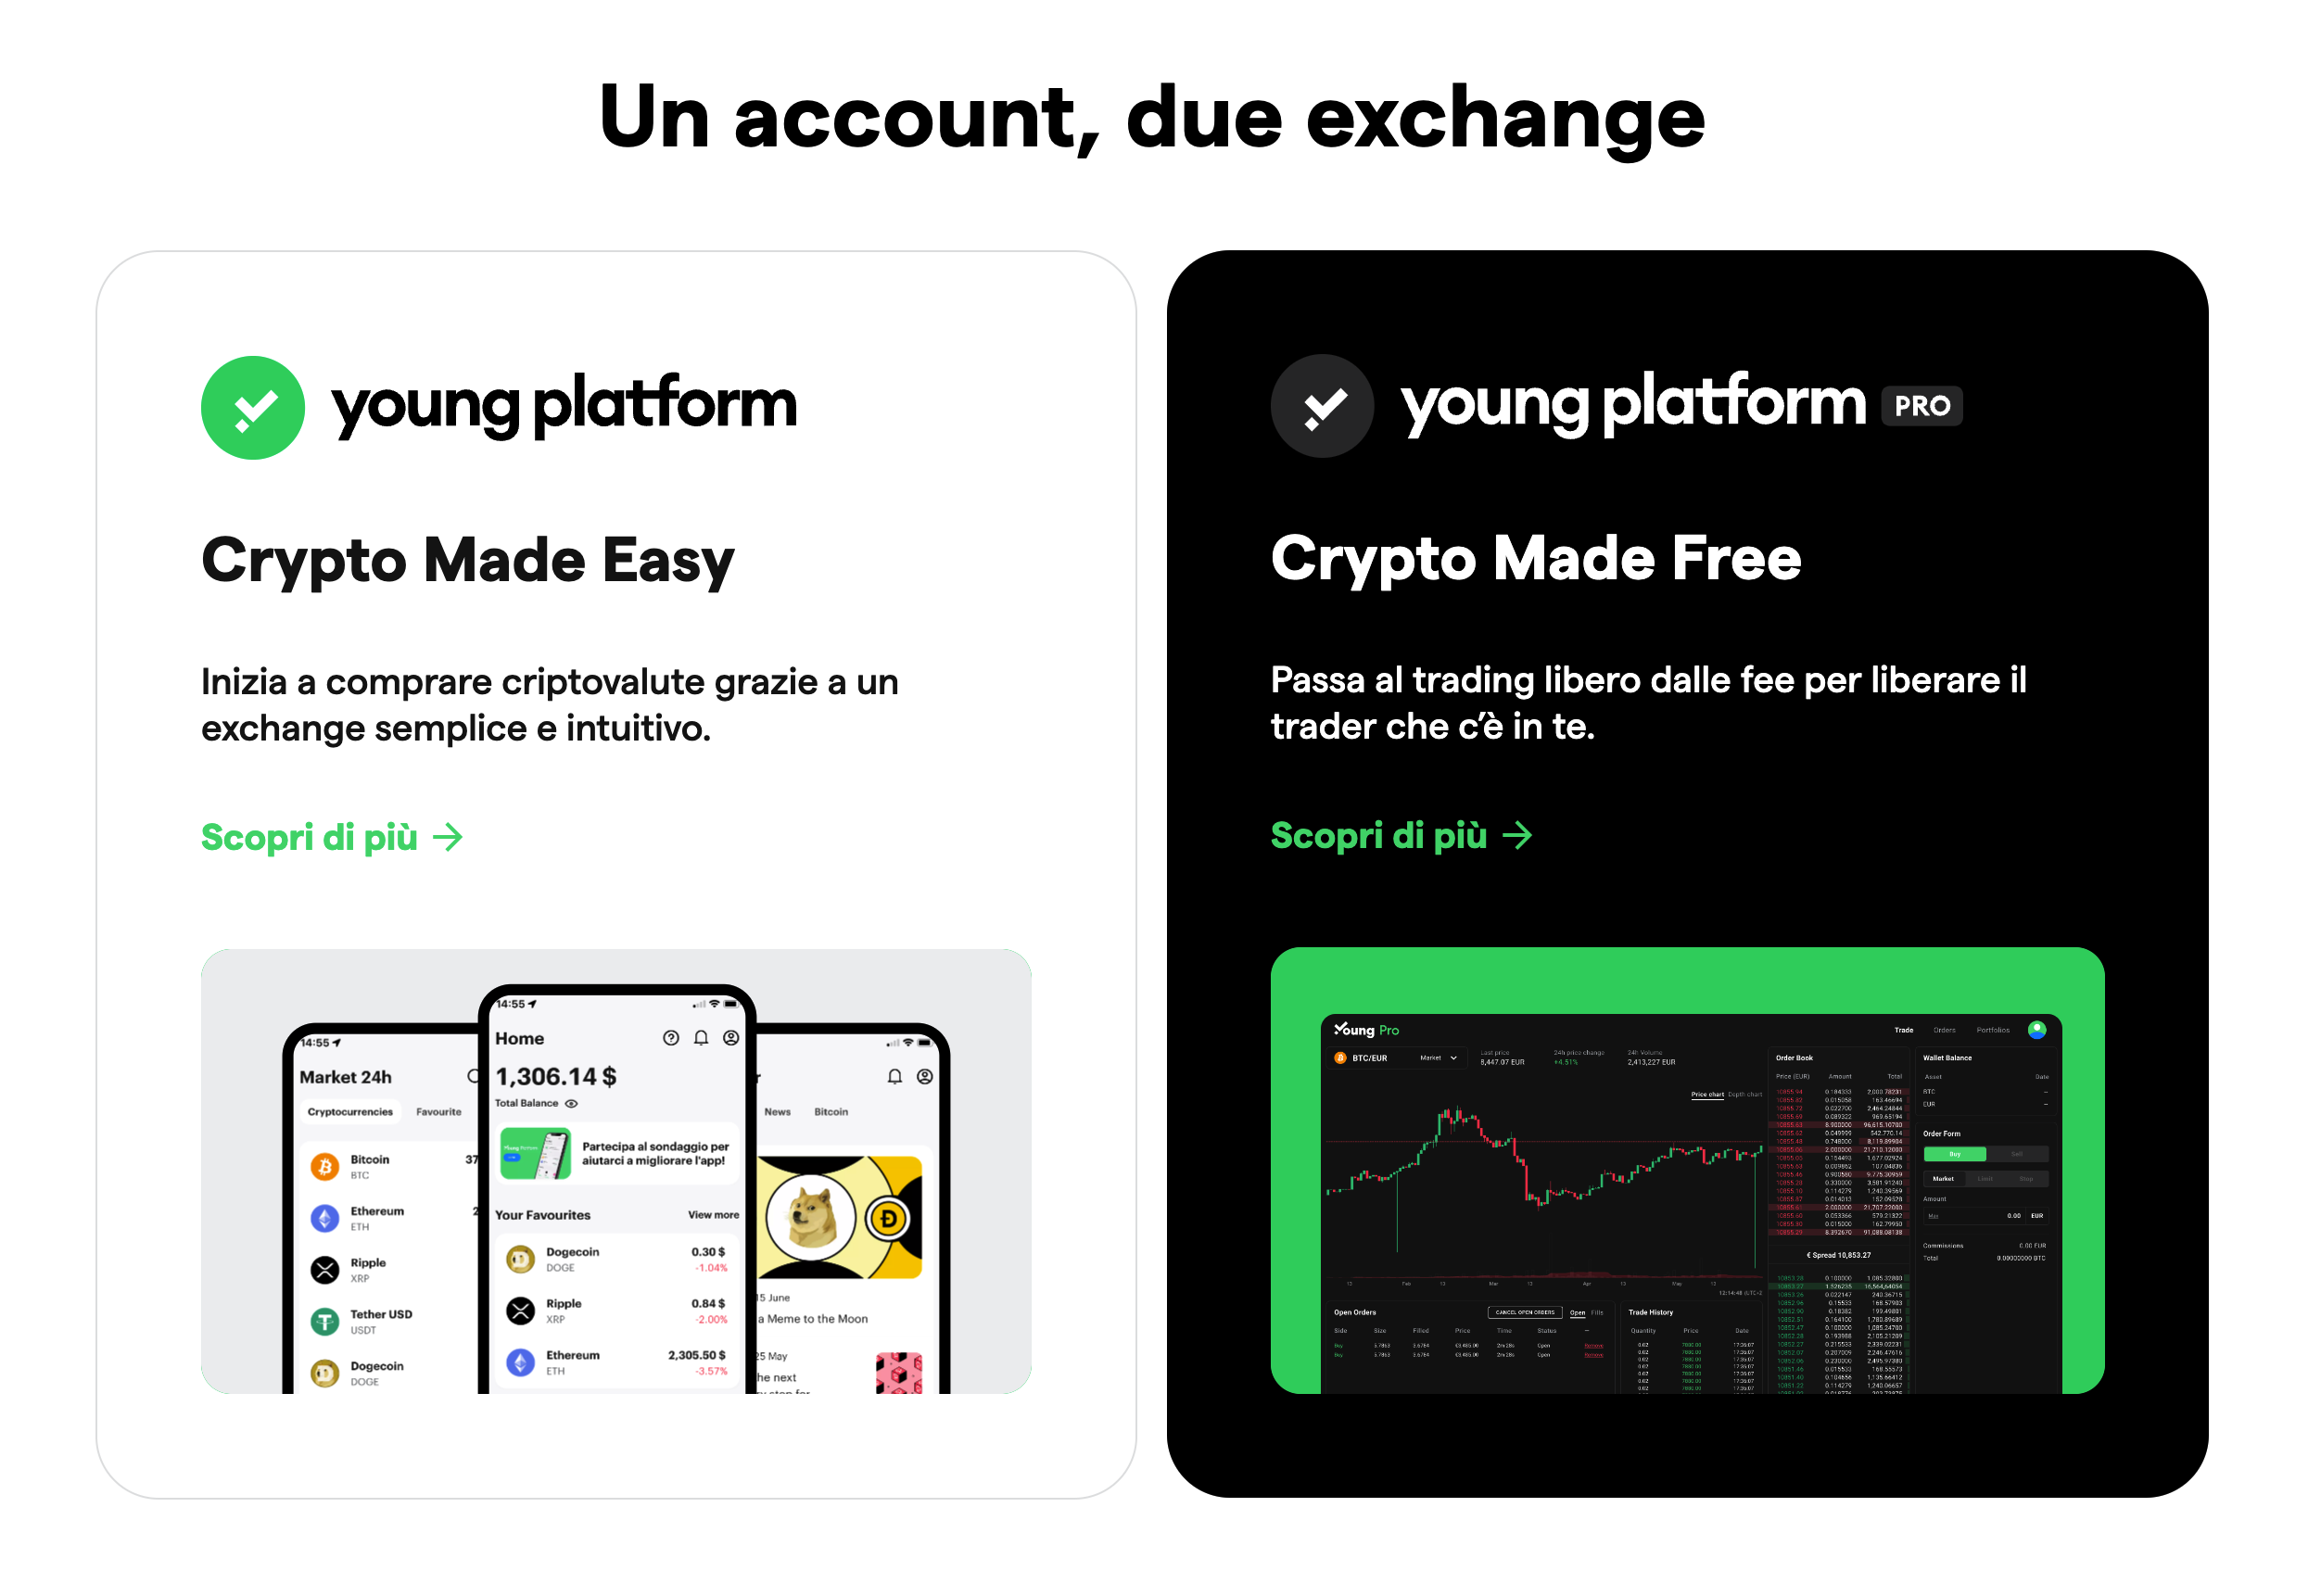
\includegraphics[width=0.80\textwidth]{res/images/internal-pages/products-page/products-page-2.png}
  \caption{Second section of the product page.}
  \label{fig:products-page-2}
\end{figure}

\begin{figure}[H]
  \centering
  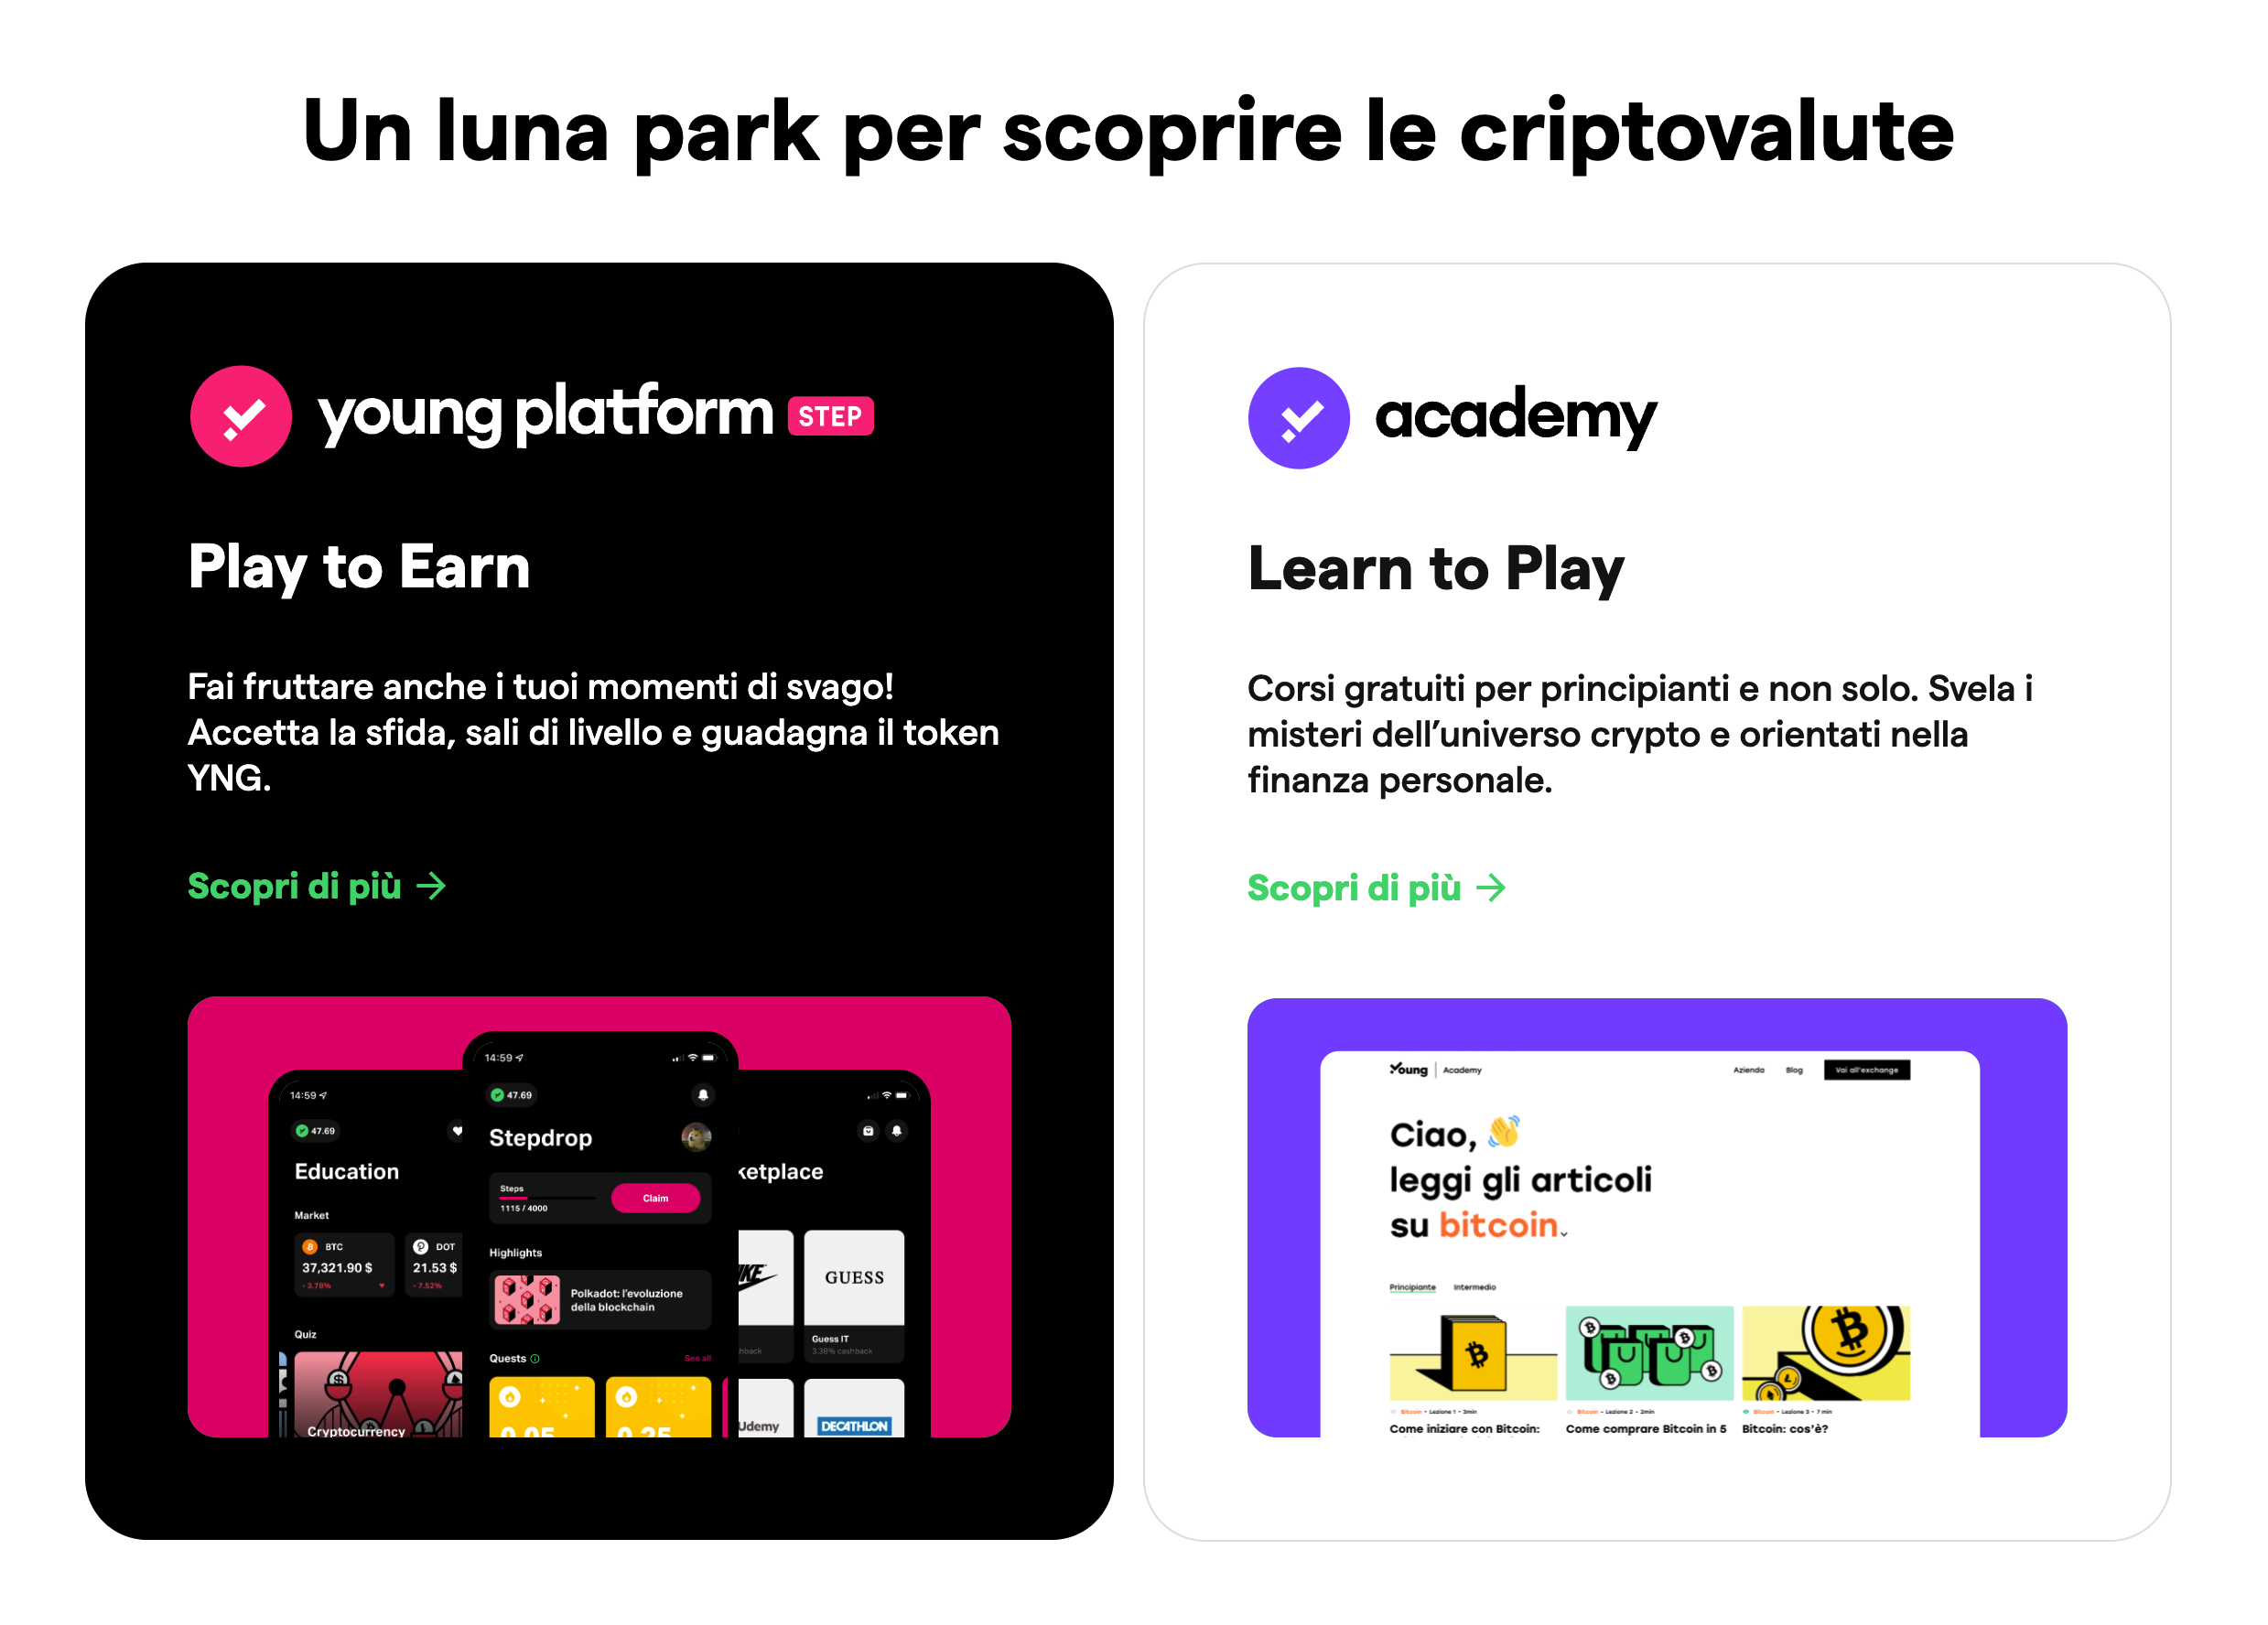
\includegraphics[width=0.80\textwidth]{res/images/internal-pages/products-page/products-page-3.png}
  \caption{Third section of the product page.}
  \label{fig:products-page-3}
\end{figure}

\paragraph{Who}

The company logo is always present at the top left, as shown in the figure 
\ref{fig:products-page-1}.

\paragraph{Where}

On this page there is a \textit{breadcrumb} and it allows the user not to 
be confused. The use of this element allows to effectively communicate most 
of the axis where (top left, under the company logo, fig. 
\ref{fig:products-page-1}).

\paragraph{Why}

The page provides excellent reasons to continue exploring it. Especially 
for a beginner user, this page represents a compass to orientate towards 
the world of cryptocurrencies and to explore the various products.

\paragraph{When}

This page has no time reference. Therefore, it is difficult for the user 
to understand if the products shown are up to date.

\paragraph{How}

This page is difficult to reach as to get to this page you need to go to 
the footer and click on \textit{I nostri prodotti} (\textit{Our products}) 
(fourth item in the third column, fig. \ref{fig:footer}). This represents a 
major disadvantage for the user.

\subsubsection{Academy page}

The page can be reached at the following address: 
\href{https://academy.youngplatform.com/}{https://academy.youngplatform.com/}.

\paragraph{What}

The purpose of this page is understandable. The purpose of this page is to 
offer a series of contents to educate and inform the user 
(fig. \ref{fig:academy-1} and \ref{fig:academy-2}). The articles are 
grouped into macro-categories (for example the \textit{Blockchain} category 
in figure \ref{fig:academy-2}) and allows to guide the user to what content 
he wishes to consult.

\begin{figure}[H]
  \centering
  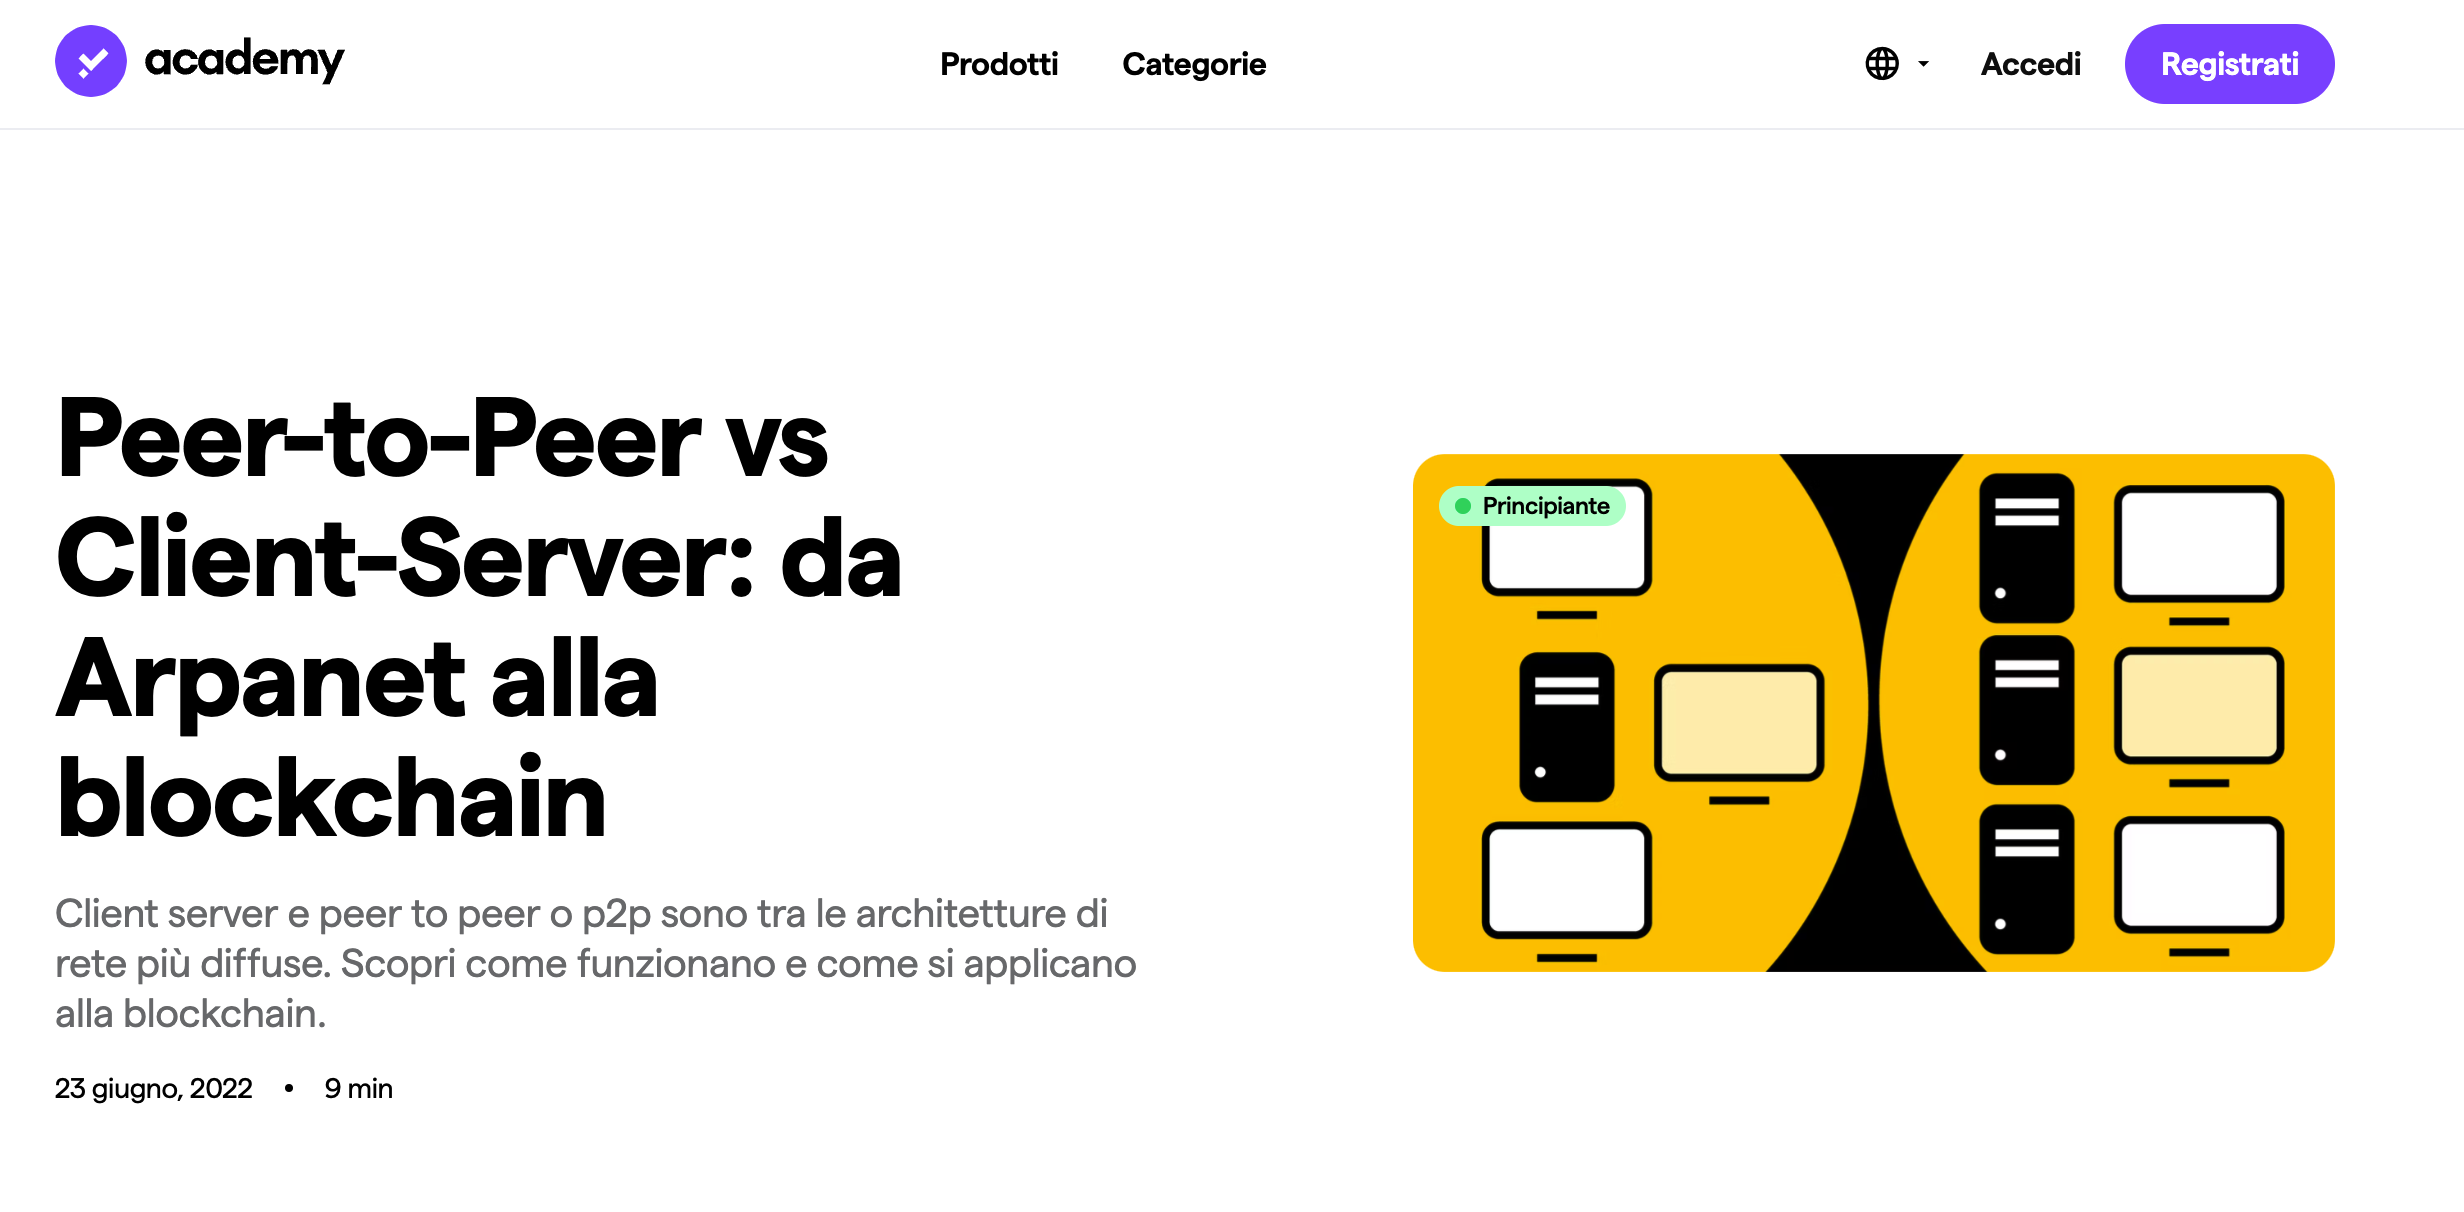
\includegraphics[width=0.80\textwidth]{res/images/internal-pages/academy/academy-1.png}
  \caption{First section of the page \textit{Academy}.}
  \label{fig:academy-1}
\end{figure}

\begin{figure}[H]
  \centering
  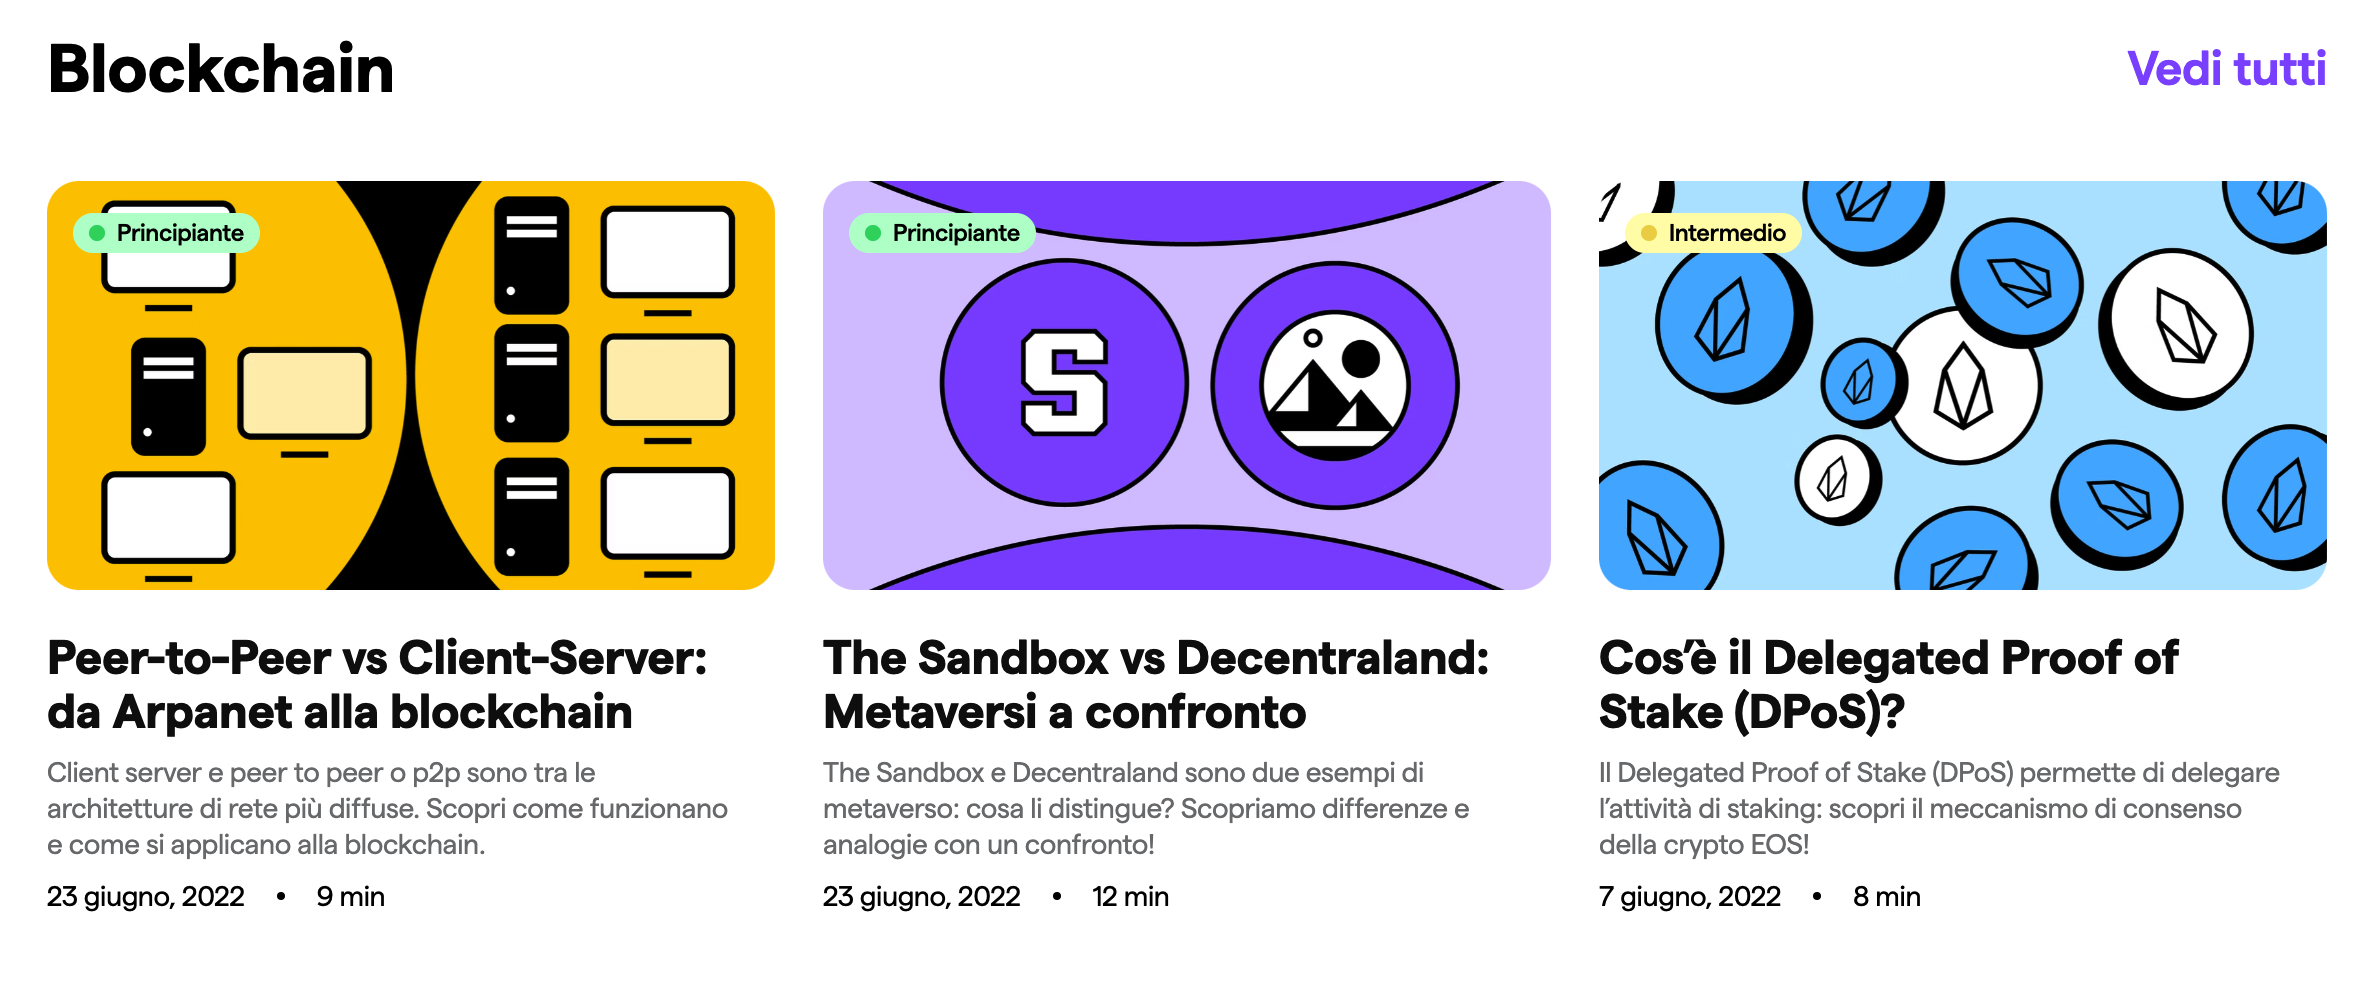
\includegraphics[width=0.80\textwidth]{res/images/internal-pages/academy/academy-2.png}
  \caption{First category of the page \textit{Academy}.}
  \label{fig:academy-2}
\end{figure}

\paragraph{Who}

The company logo is present at the top left, as shown in figure 
\ref{fig:academy-1}. However, it has a different color than the original 
color (green). The company has chosen to color the logo with a different 
color for each product. The user is still able to recognize the logo 
itself, even if it is not the original color. 

\paragraph{Where}

When the user is redirected to this page, they may notice that they have 
arrived at a new subdomain (\textit{academy.youngplatform.com}). However, 
there is no element that allows you to return to the page you have 
reached or to return to the \textit{youngplatform.com} homepage. In order 
to return to the homepage, you need to go to the footer. This 
implementation is very disadvantageous for the user and requires some 
effort to perform the action.

\paragraph{Why}

This page offers some great reasons to explore it:
\begin{itemize}
  \item For beginner users it is possible to draw on a large number of 
  articles that allow you to introduce to the world of cryptocurrencies 
  and blockchain;

  \item However, for expert users it is possible to read articles 
  concerning the latest news in the sector or articles illustrating 
  comparisons between two technologies/competitors.
\end{itemize}

Furthermore, it is possible to note that the element representing the 
article is composed of an image, a title, a short introduction description 
and time references. At the top left of the image there is an element 
that indicates who this article is for, that is, the articles are divided 
between \textit{Principiante} (\textit{Beginner}), \textit{Intermedio} 
(\textit{Intermediate}) and \textit{Esperto} (\textit{Expert}). 
This strategy is very useful as it allows a user to choose articles that 
match their experience in the sector.

\paragraph{When}

In this page there are clear time references: it is possible to note that 
for each article on the page there is the publication date of the article 
(fig. \ref{fig:academy-1} and \ref{fig:academy-2}). Furthermore, as shown 
in the figure \ref{fig:academy-1}, the last published article is inserted 
in the initial section of this page, in order to highlight it.

\paragraph{How}

This page is easy to reach, as it is sufficient to go to the main menu of 
\textit{youngplatform.com} under \textit{Prodotti} (\textit{Products}). 
This page can also be reached via the footer.

\newpage

\subsubsection{Academy - Blockchain}

The page can be reached at the following address: 
\href{https://academy.youngplatform.com/blockchain/}{https://academy.youngplatform.com/blockchain/}. 

\paragraph{What}

This page explicitly states what is being offered, that is, a series of 
articles are offered that deal with topic \textit{Blockchain}. 

\begin{figure}[H]
  \centering
  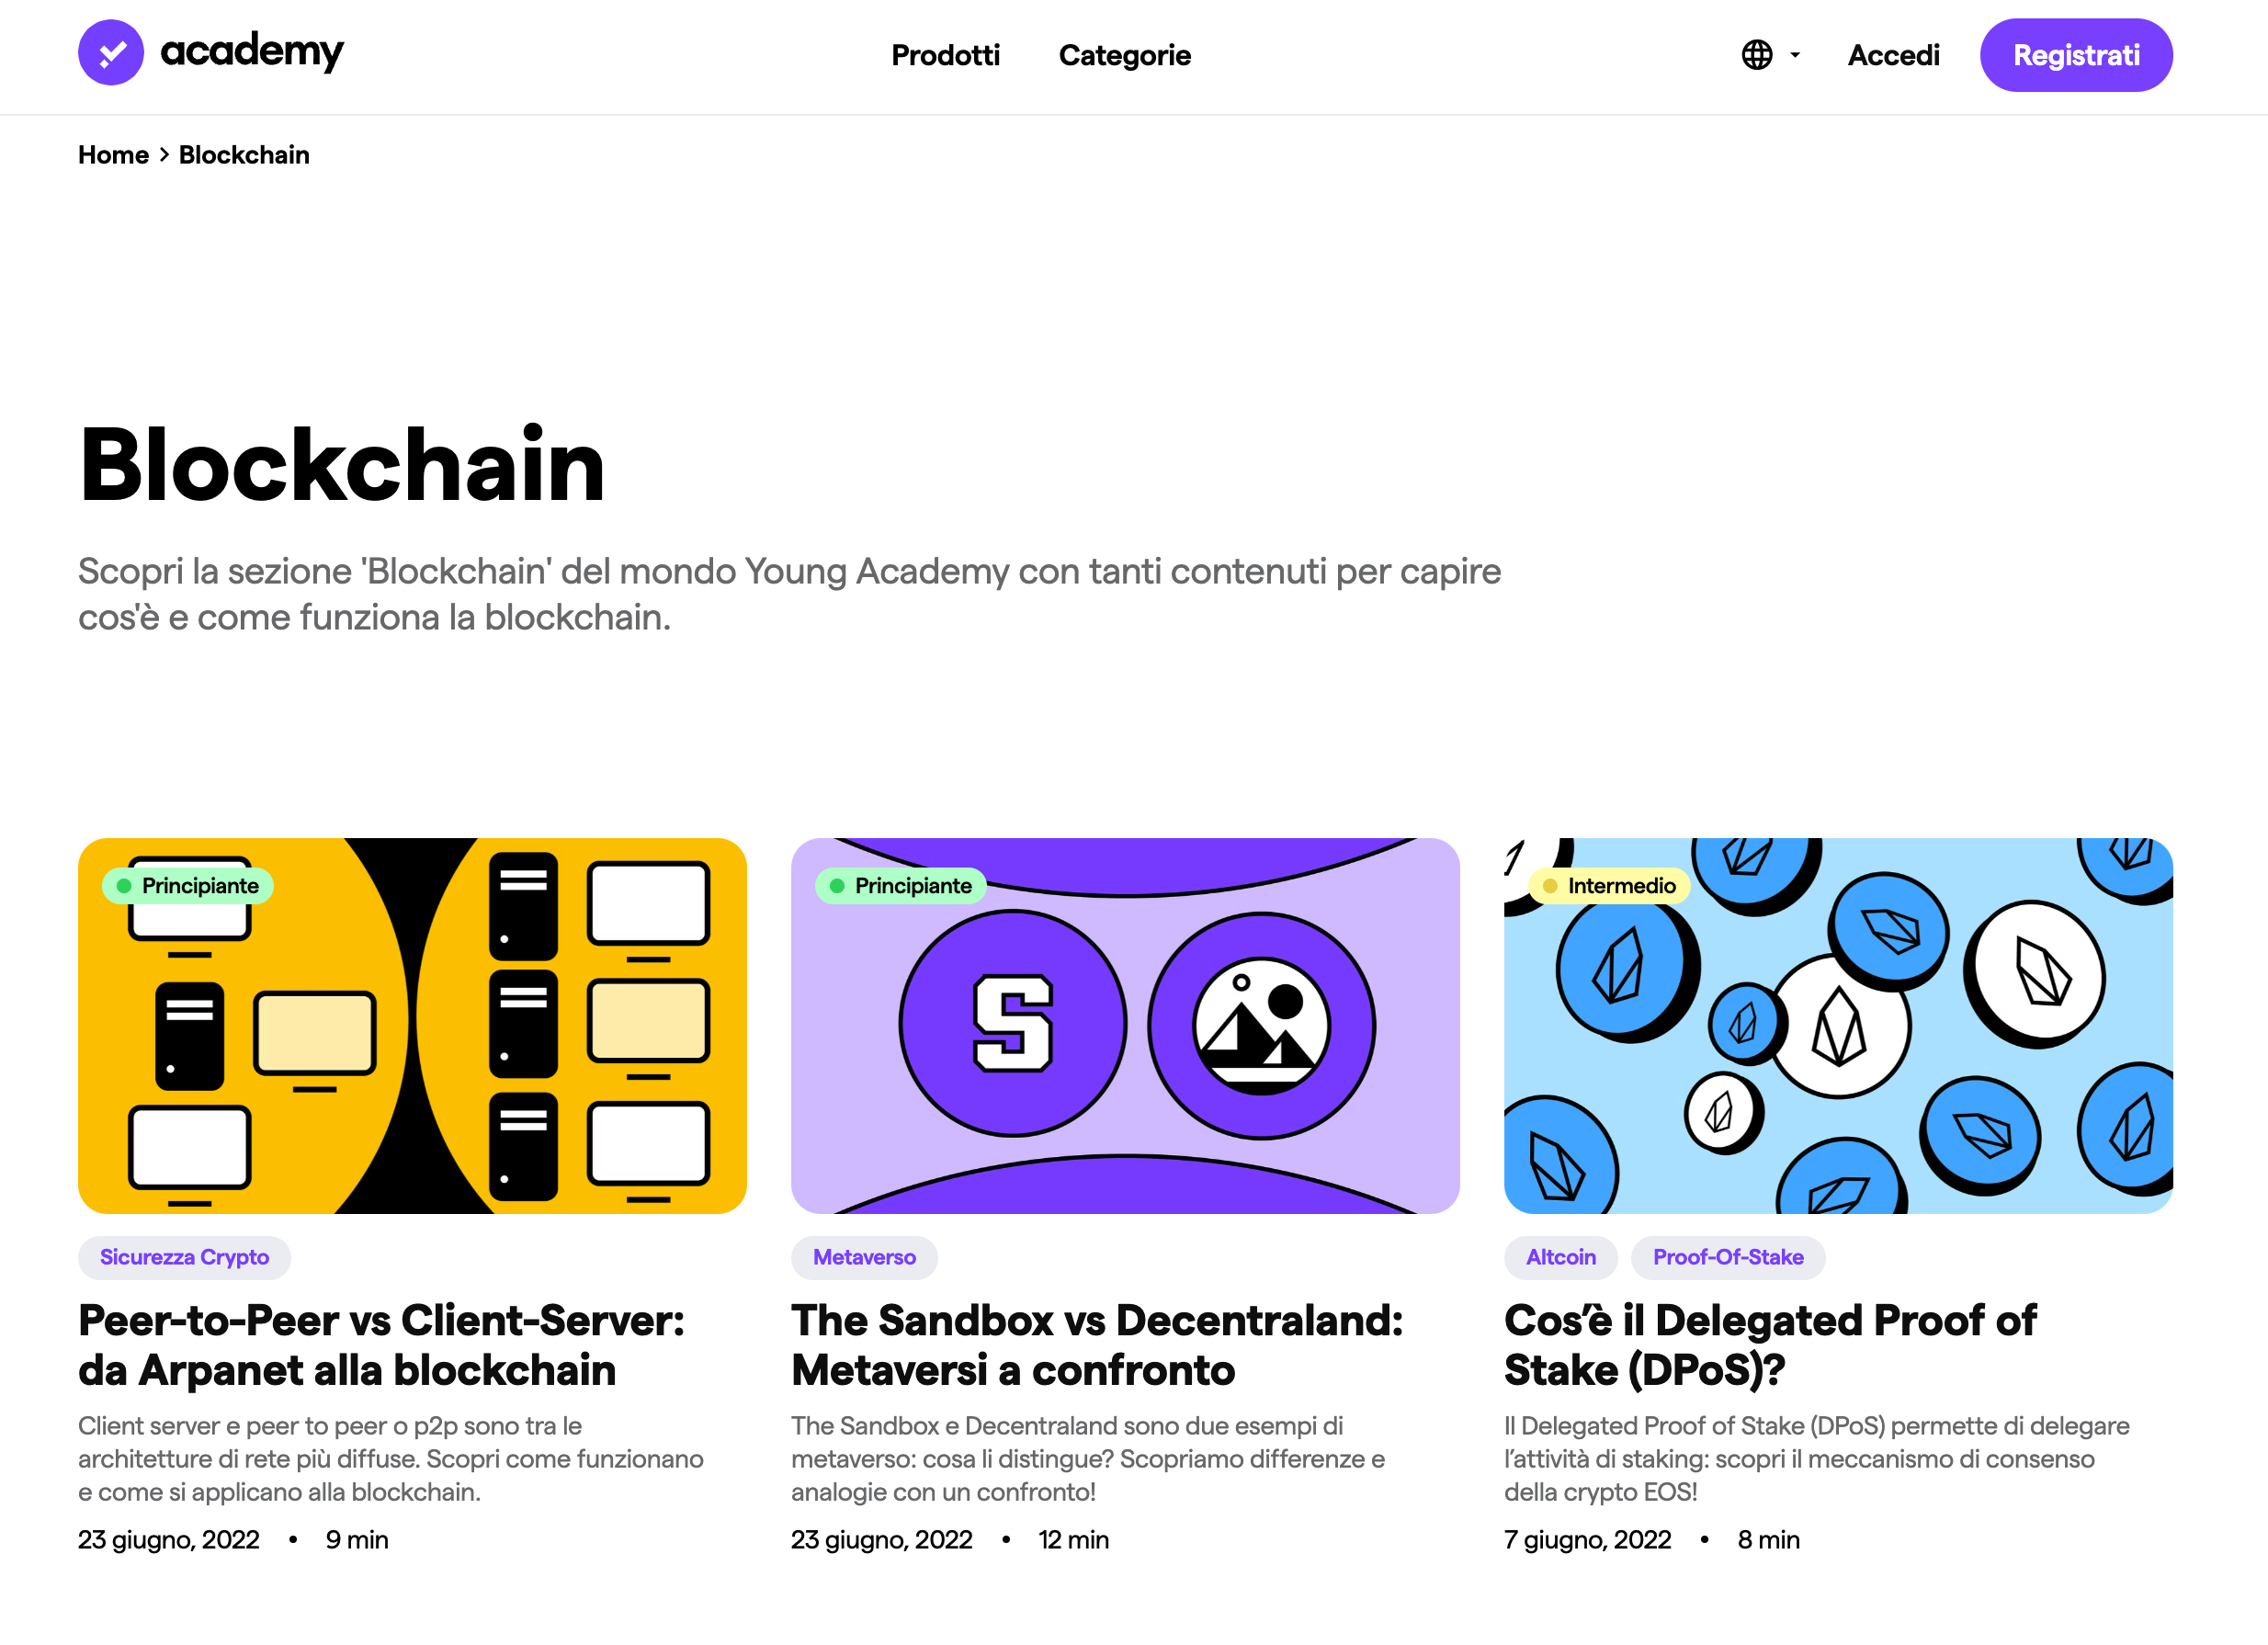
\includegraphics[width=0.80\textwidth]{res/images/internal-pages/academy/academy-3.png}
  \caption{Section of articles from the \textit{Blockchain} category.}
  \label{fig:academy-3}
\end{figure}

\paragraph{Who}

The company logo is present at the top left, as shown in the figure 
\ref{fig:academy-3}.

\paragraph{Where}

On this page there is a \textit{breadcrumb} and it allows the user not to 
be confused. The use of this element allows to effectively communicate 
most of the where axis (top left, under the company logo, fig. 
\ref{fig:academy-3}). It is also possible to notice that at the end of the 
page in the figure \ref{fig:academy-4} (bottom right) there is an element 
called \textit{Precedenti} (\textit{Previous}). This element tells the user 
that the contents are \textit{paginated}, that is, each page has a certain 
number of articles. If you want to search for an older article, the site 
offers a way to browse and search for other articles.

\begin{figure}[H]
  \centering
  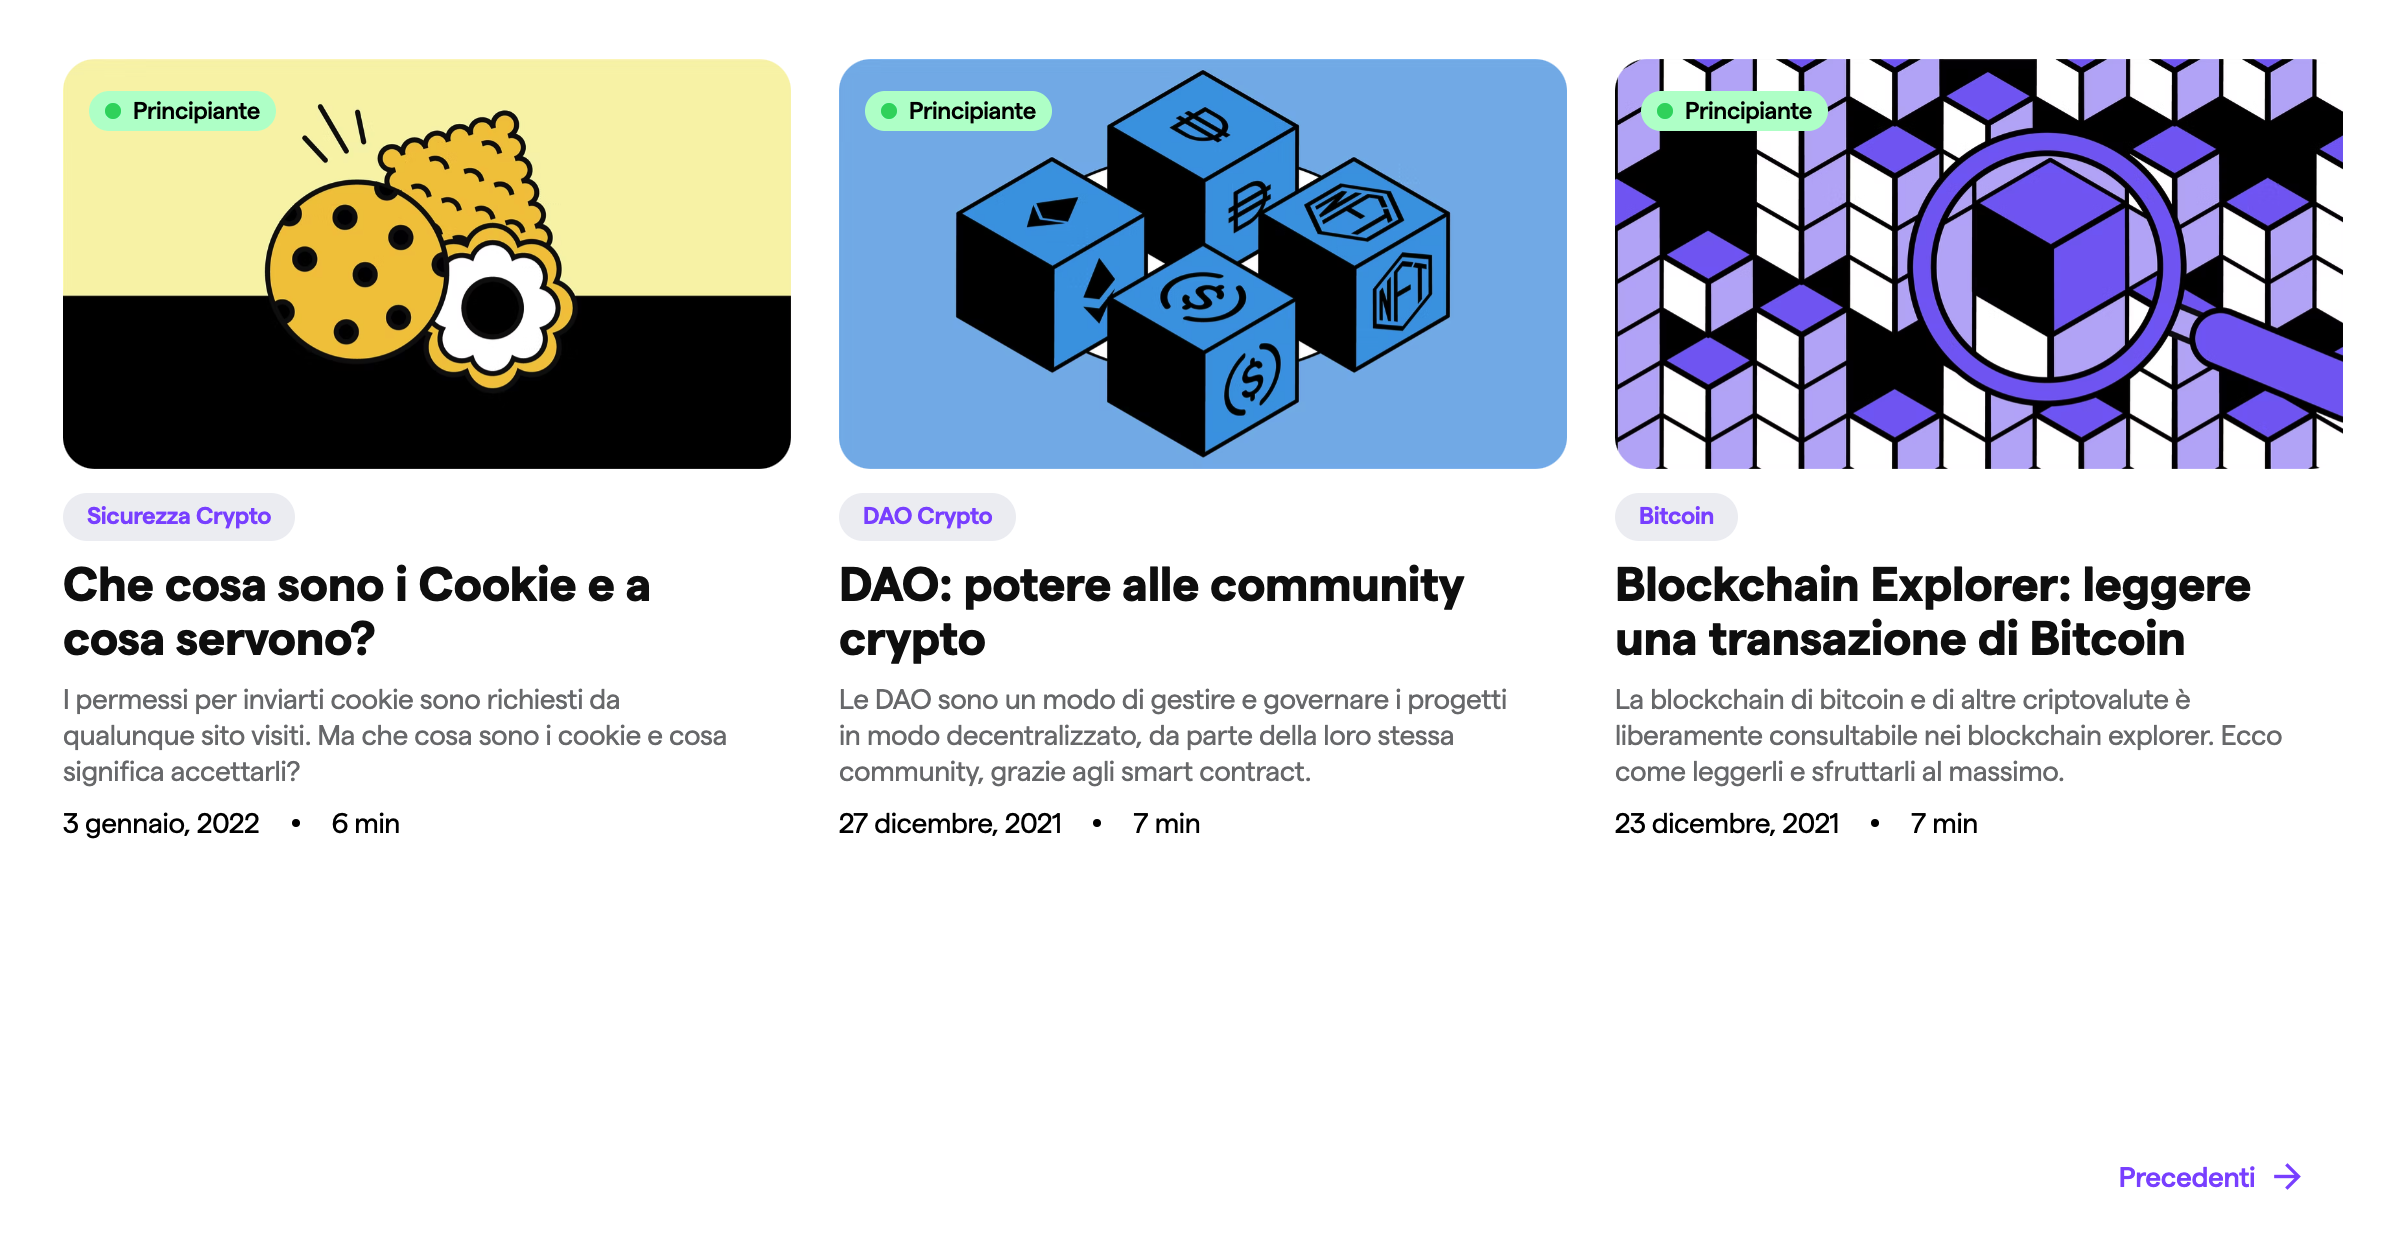
\includegraphics[width=0.80\textwidth]{res/images/internal-pages/academy/academy-4.png}
  \caption{End of page of the \textit{Blockchain} category.}
  \label{fig:academy-4}
\end{figure}

\paragraph{Why}

This page offers different reasons to continue exploring it. If the user 
is inexperienced in the field, then the user will want to read several 
articles and explore the page to search for introductory content. If the 
user is an expert, the user will explore the page to search for a specific 
article, in order to directly obtain the information sought.

\paragraph{When}

On this page there are time references: it is possible to note that for 
each article on the page there is the date of publication of the article 
(fig. \ref{fig:academy-3}).

\paragraph{How}

This page is not easy to reach as it represents a specific category of 
articles. Therefore, if the user needs information regarding this topic, 
he will have to carry out a search. In this particular case, this page can 
be reached from the page 
\href{https://academy.youngplatform.com/}{https://academy.youngplatform.com/}, 
by clicking on \textit{Vedi tutti} (\textit{See all}) (located at the top 
right, colored purple).

\subsubsection{Academy - Blockchain - Article}

The page can be reached at the following address: \\
\href{https://academy.youngplatform.com/blockchain/peer-to-peer-p2p-client-server-cosa-sono-come-funzionano/}{https://academy.youngplatform.com/blockchain/peer-to-peer-p2p-client-server-cosa-sono-come-funzionano/}.

\paragraph{What}

This page explicitly states the content that is offered to the user, in 
particular, in that page, a very specific content that has been chosen by 
the user will be offered.

\begin{figure}[H]
  \centering
  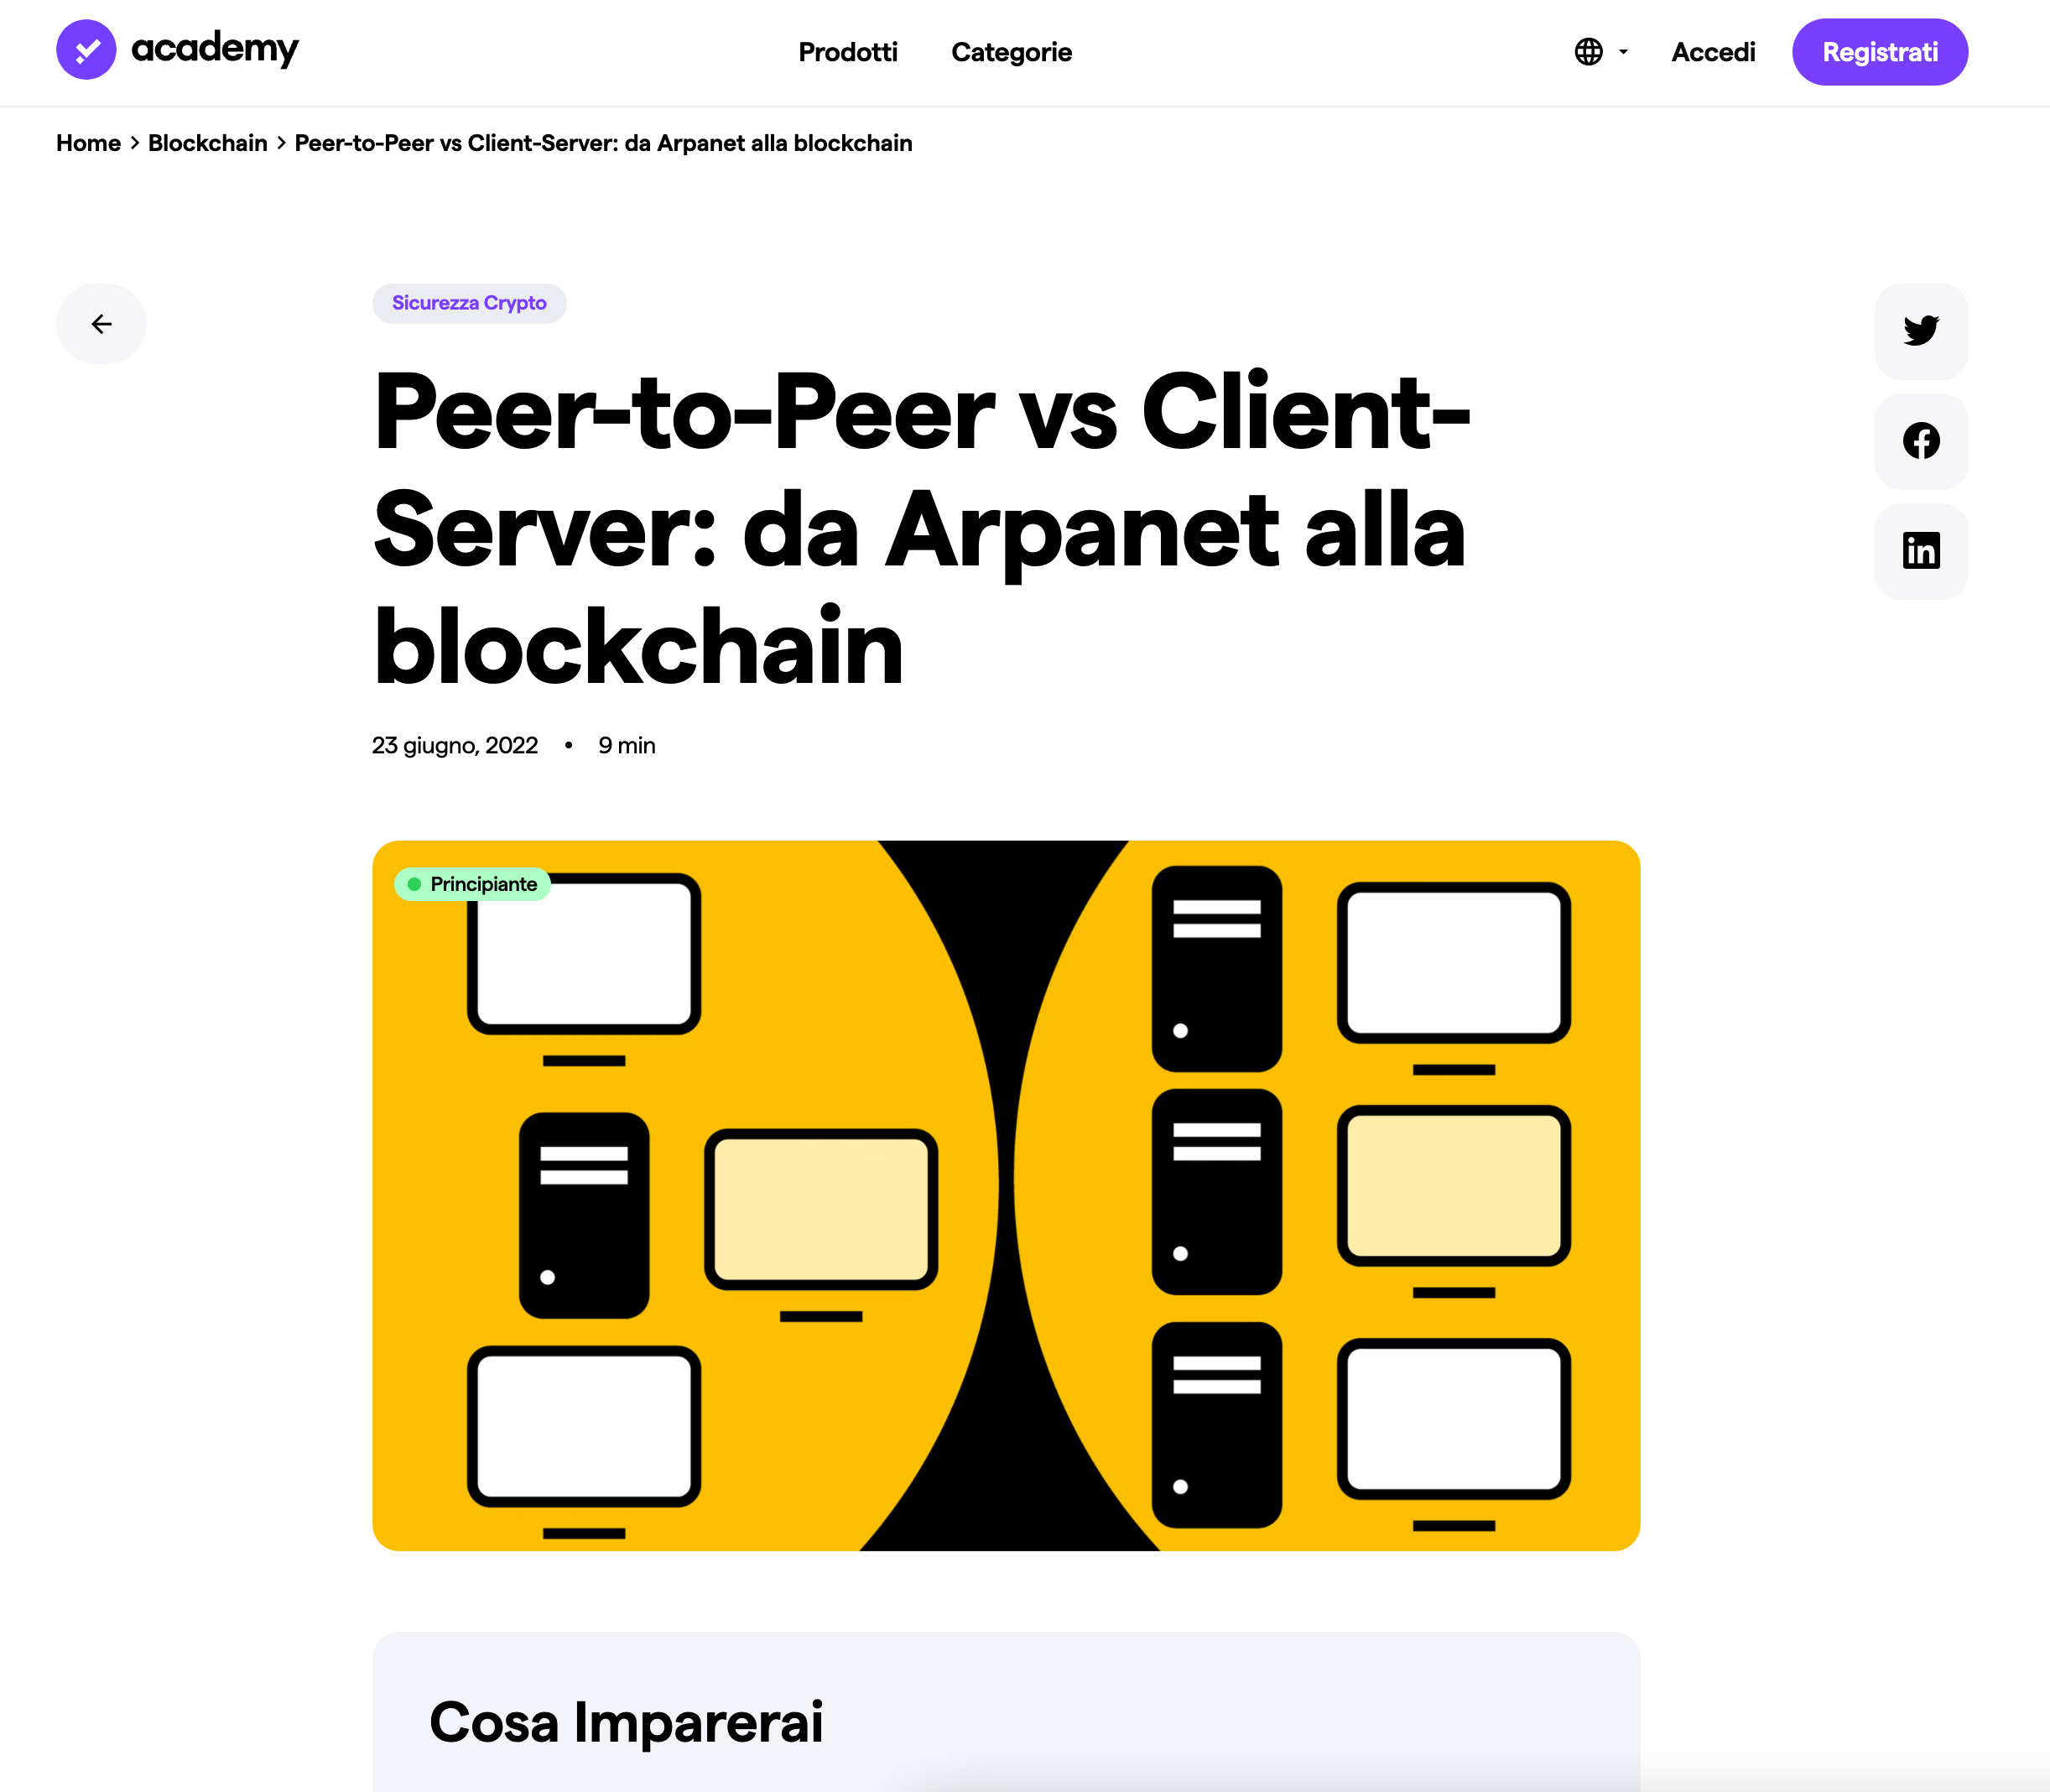
\includegraphics[width=0.80\textwidth]{res/images/internal-pages/academy/academy-5.png}
  \caption{An article from the \textit{Blockchain} category.}
  \label{fig:academy-5}
\end{figure}

\paragraph{Who}

The company logo is present at the top left, as shown in the figure 
\ref{fig:academy-5}.

\paragraph{Where}

Also on this page there is a \textit{breadcrumb} and it allows the user 
not to be confused. The use of this element allows to effectively 
communicate  most of the where axis (top left, under the company logo, 
fig. \ref{fig:academy-5}). It is also possible to notice that in figure 
\ref{fig:academy-6}, under the company logo, there is a purple bar. This 
bar indicates at what point the user is reading the article. So, in 
particular, the length of the purple bar indicates the portion of text 
that has been read. This element is very useful for the user as he can 
actually realize the length of the article.

\begin{figure}[H]
  \centering
  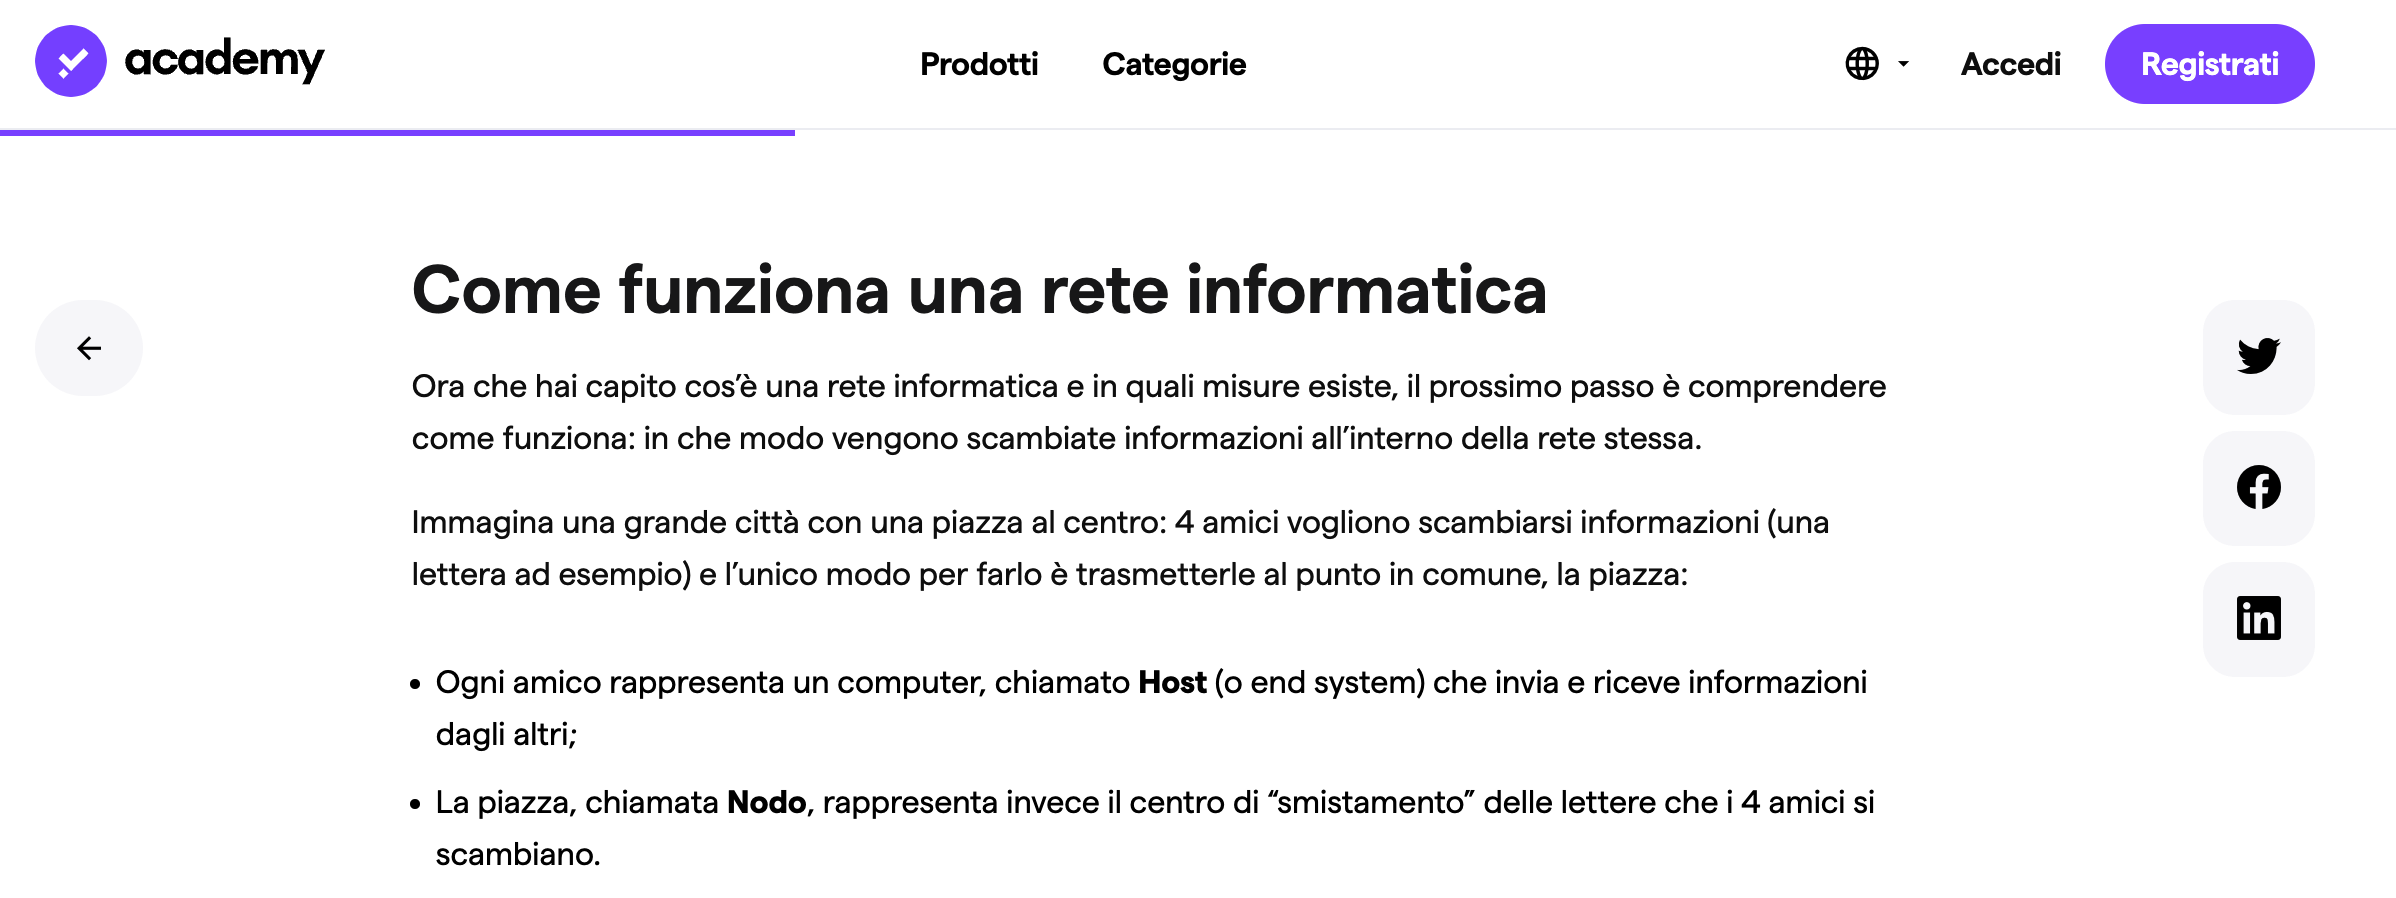
\includegraphics[width=0.80\textwidth]{res/images/internal-pages/academy/academy-6.png}
  \caption{Dynamic bar that indicates how far you have reached with the 
  reading of the article.}
  \label{fig:academy-6}
\end{figure}

There is another element on the page that increases the usability of the 
site: in the figure \ref{fig:academy-5} on the left there is an arrow that 
allows you to go back, in the list of articles of the 
\textit{Blockchain category}. This element always remains in the same 
position even if the user scrolls the page (see also figure 
\ref{fig:academy-6}). This is a positive aspect because if the user wants 
to return to the previous page, it is not necessary for the user to return 
to the top of the page.

\paragraph{Why}

The main reason the user should explore the page is that he is directly 
interested in this article. At the end of the page, the site offers, in a 
special section, additional articles related to the one just read 
(fig. \ref{fig:academy-7}). This provides one more reason to continue 
browsing the site.

\begin{figure}[H]
  \centering
  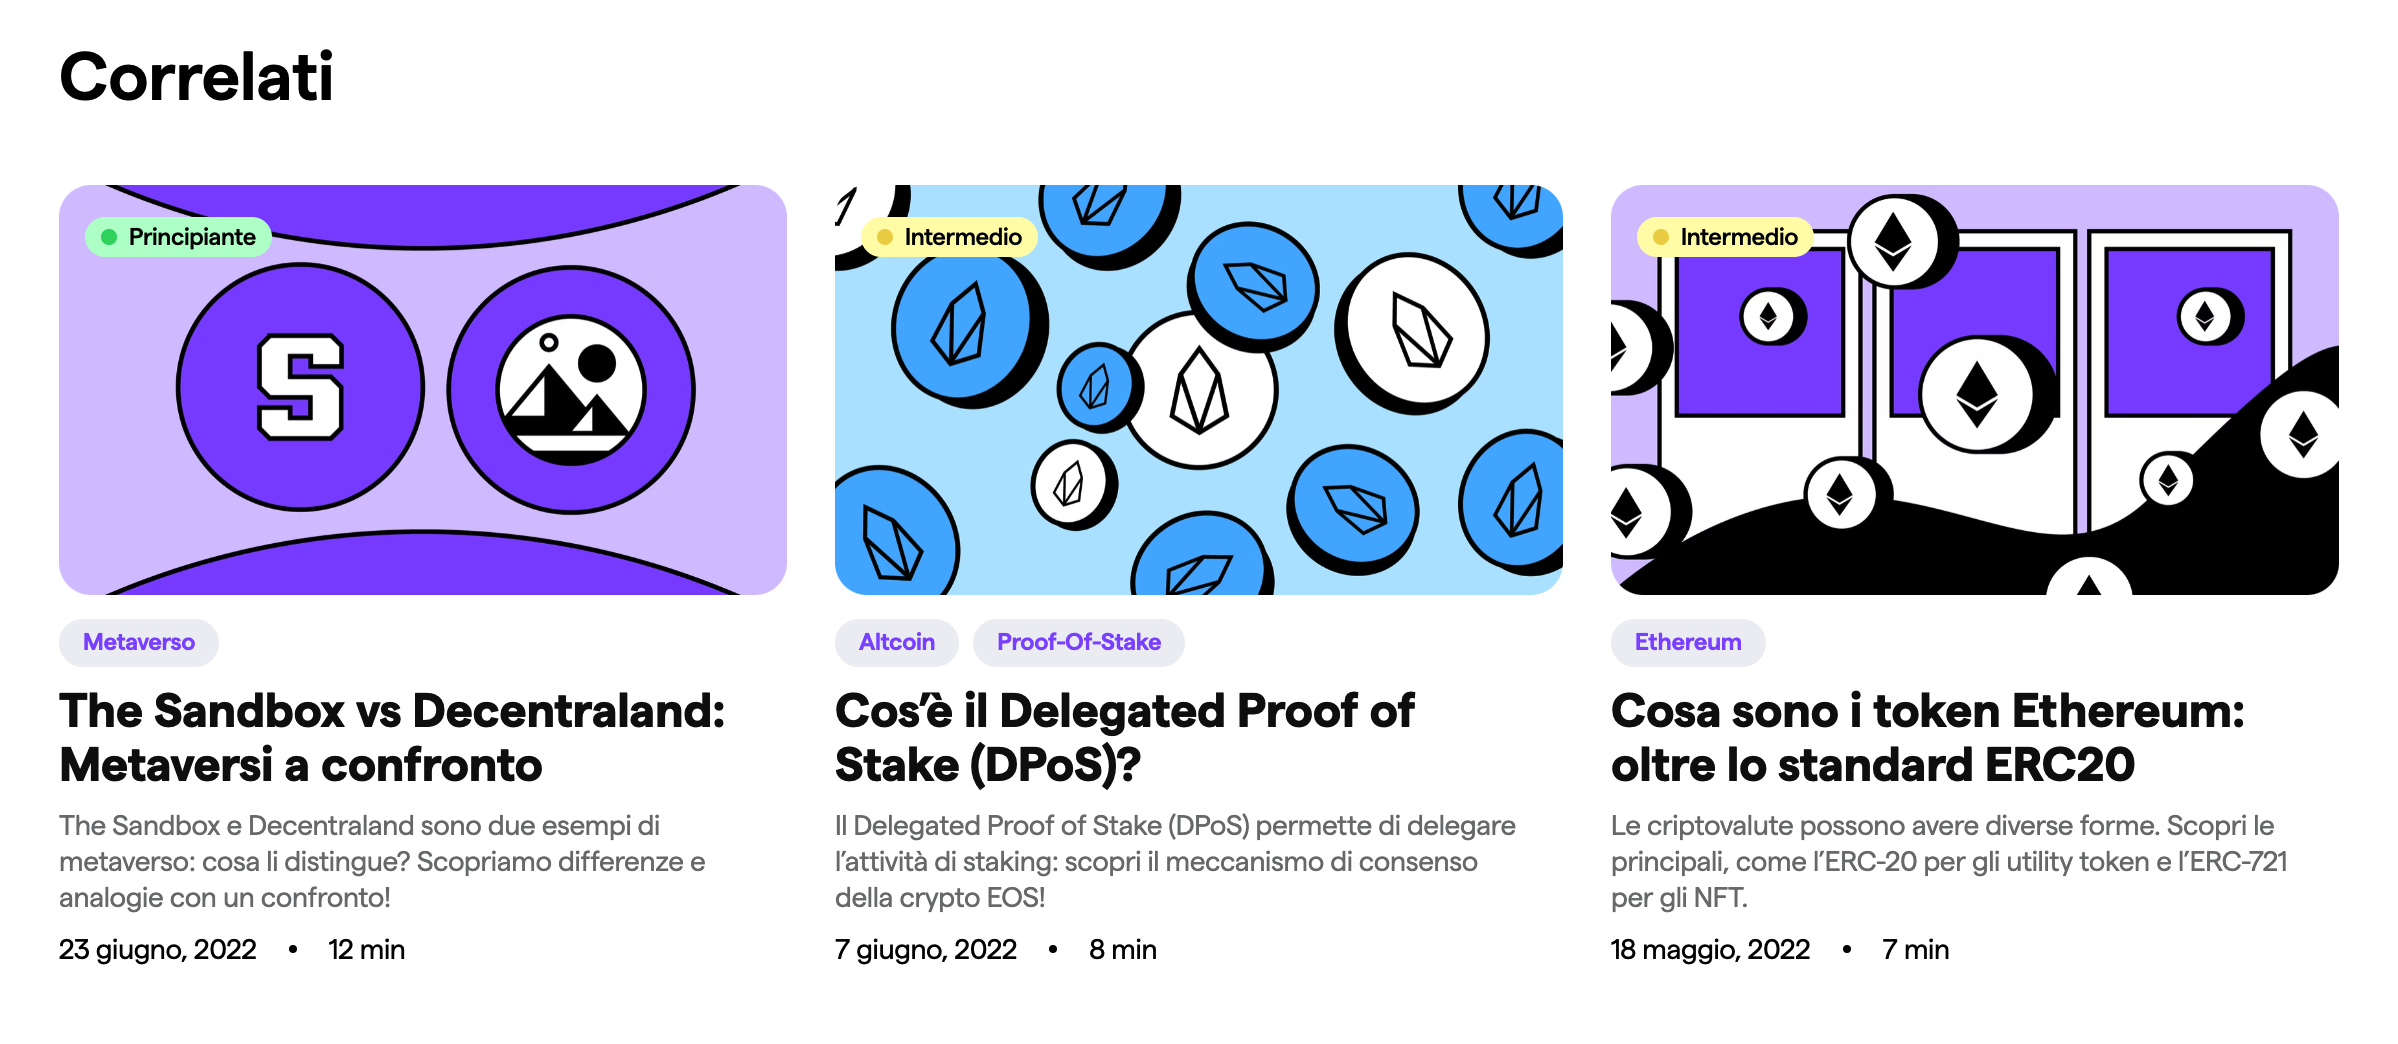
\includegraphics[width=0.80\textwidth]{res/images/internal-pages/academy/academy-7.png}
  \caption{End of article page.}
  \label{fig:academy-7}
\end{figure}

\paragraph{When}

On this page there is a time reference and it is possible to locate it 
under the title of the article (fig. \ref{fig:academy-5}).

\paragraph{How}

This page is not easy to reach, as the user must actually be interested in 
that article. Therefore, the user will have to search to find such an 
article. Unfortunately, the search must be done through a search engine, 
or the user should explore the previous page to find the article. This 
page can be reached via 
\href{https://academy.youngplatform.com/blockchain/}{https://academy.youngplatform.com/blockchain/}.

\subsubsection{Glossary page}

The page can be reached at the following address: 
\href{https://youngplatform.com/glossary/}{https://youngplatform.com/glossary/}.

\paragraph{What}

The content of this page is explicitly stated, that is, the objective of 
this page is to enclose a set of technical terms of the sector and to 
provide a description for each of them.

\begin{figure}[H]
  \centering
  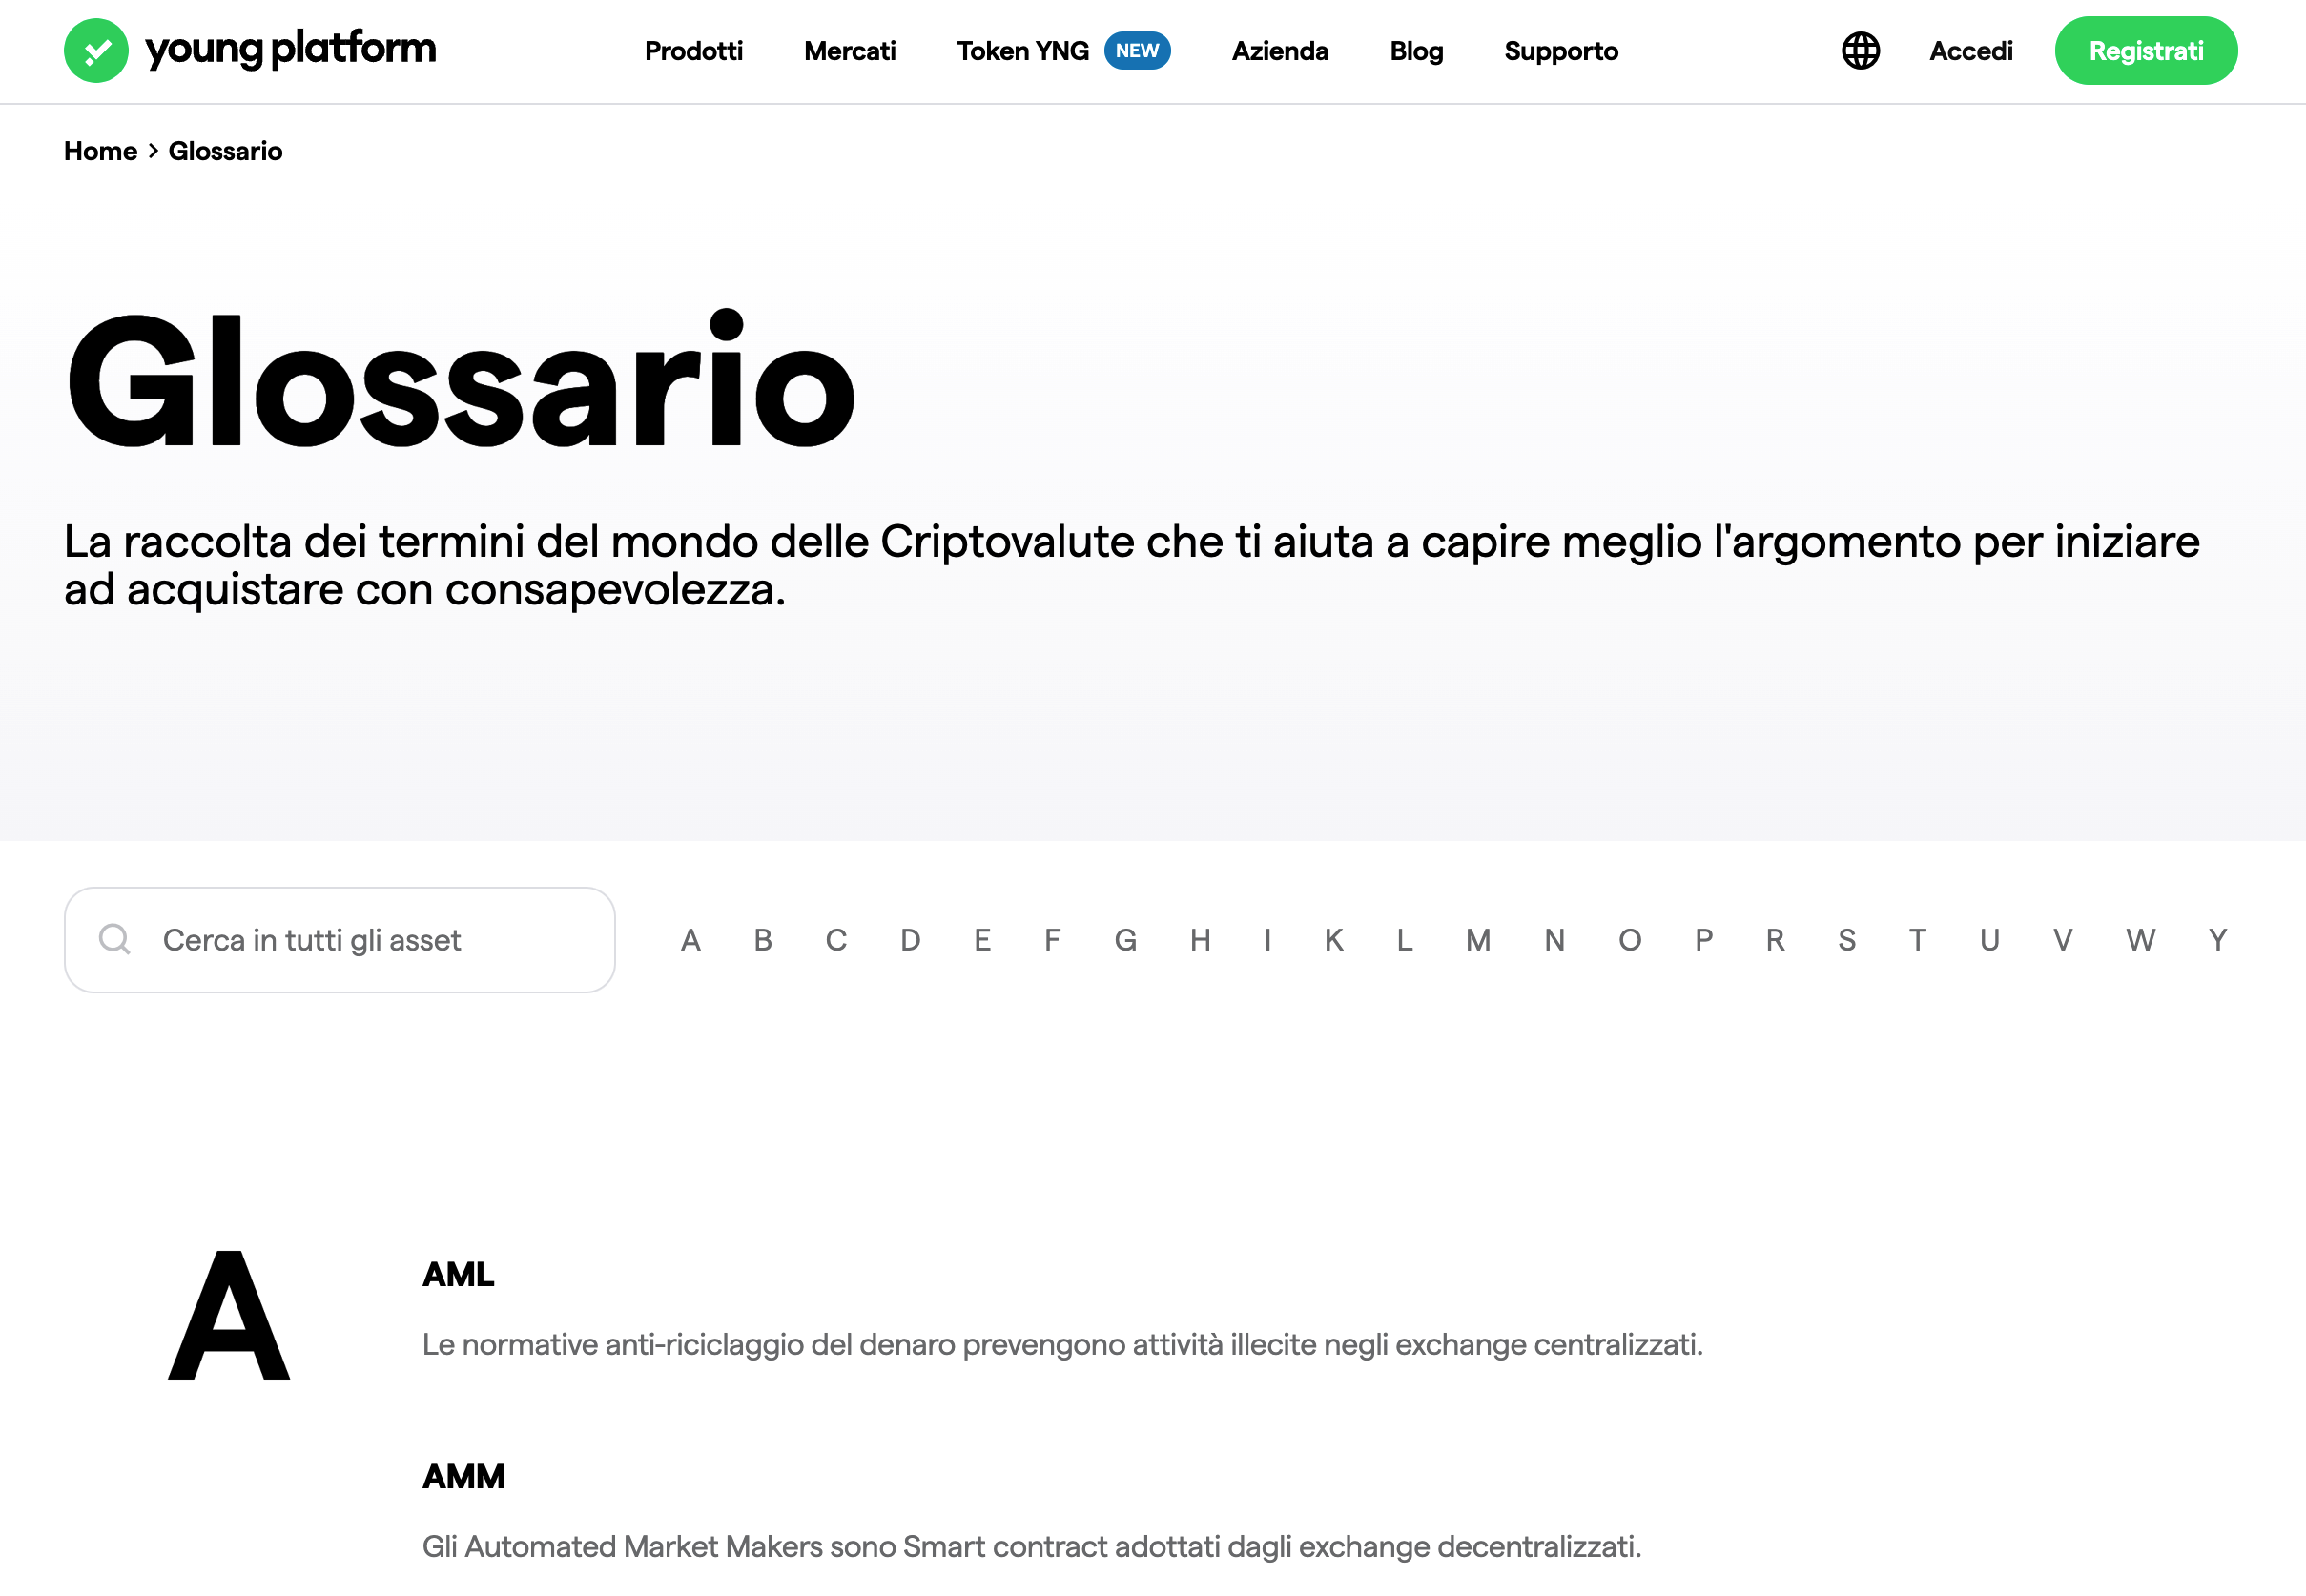
\includegraphics[width=0.80\textwidth]{res/images/internal-pages/glossary/glossary-1.png}
  \caption{Glossary page.}
  \label{fig:glossary-1}
\end{figure}

\paragraph{Who}

The company logo is always present at the top left, as shown in the figure 
\ref{fig:glossary-1}.

\paragraph{Where}

Also on this page there is a \textit{breadcrumb} and it allows the user not 
to be confused. The use of this element allows to effectively communicate 
most of the where axis (top left, under the company logo, fig. 
\ref{fig:glossary-1}).

\paragraph{Why}

A novice user has more reasons to explore this page, as it is assumed that 
for an experienced user these terms are already well known.

\paragraph{When}

There is no time reference on this page.

\paragraph{How}

This page is difficult to reach, as you have to go to the footer of the 
site (second item in the second column, fig. \ref{fig:footer}). This is an 
important disadvantage especially for a beginner user: this page, from his 
point of view, is of enormous importance, as it represents a reference 
point for understanding the meaning of a myriad of technical terms in the 
sector. Therefore, this page should be placed side by side with very 
important and useful pages (for example, the blog) and easily accessible. 
This page provides two tools for searching for specific terms (fig. 
\ref{fig:glossary-2}):

\begin{figure}[H]
  \centering
  
\includegraphics[width=0.80\textwidth]{res/images/internal-pages/glossary/glossary-2.png}
  \caption{Search tools for terms in the glossary.}
  \label{fig:glossary-2}
\end{figure}

\begin{itemize}
  \item On the left there is a search bar where the user can type in a 
  term and then find its meaning. For each character that is typed, the 
  site offers all the terms related to the characters entered up to that 
  moment, so as to also display other similar or related terms;

  \item On the right are the letters of the alphabet, each of which can be 
  clicked. If you click on one of these letters, the site will propose all 
  terms starting with that letter. In figure \ref{fig:glossary-3} you can 
  see an example. This tool is very useful for users who are not yet 
  familiar with the various terms in this industry and therefore may not 
  remember the exact name of a term.
\end{itemize}

\begin{figure}[H]
  \centering
  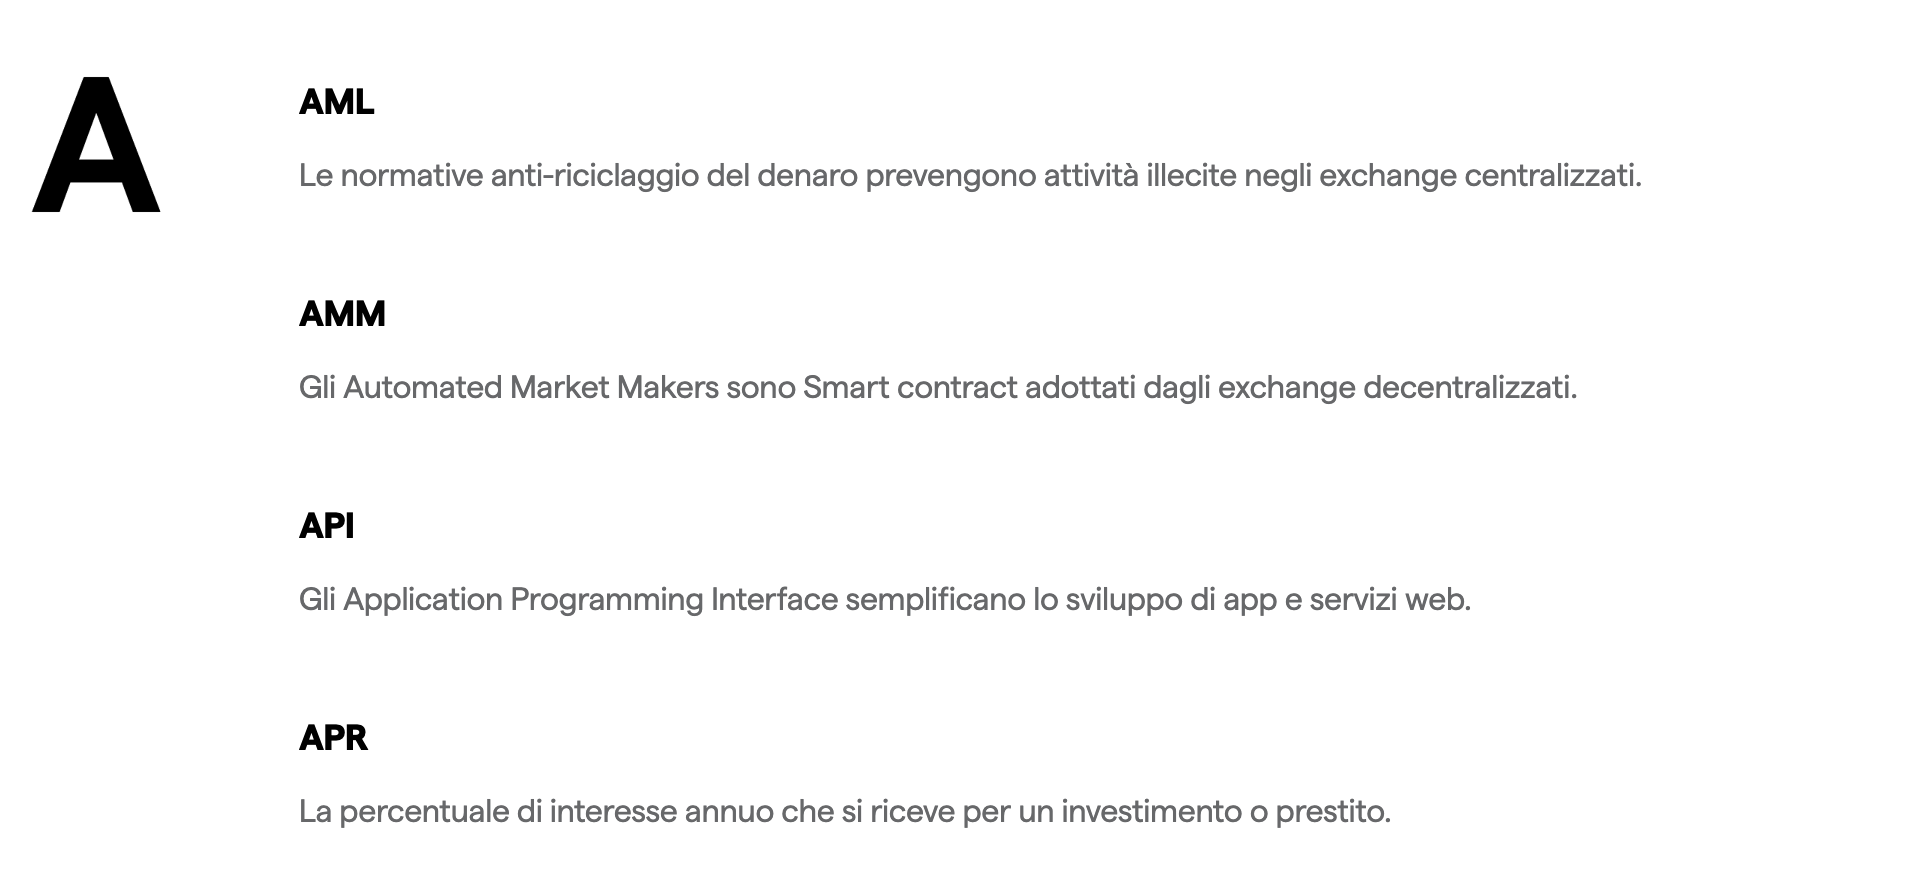
\includegraphics[width=0.80\textwidth]{res/images/internal-pages/glossary/glossary-3.png}
  \caption{Some results for the letter \textit{A}.}
  \label{fig:glossary-3}
\end{figure}

\subsubsection{Page of a term of the glossary}

The page can be reached at the following address: 
\href{https://youngplatform.com/glossary/api/}{https://youngplatform.com/glossary/api/}.

\paragraph{What}

The content of this page clearly expresses its goal, that is, to provide 
the meaning of a term previously chosen by the user.

\begin{figure}[H]
  \centering
  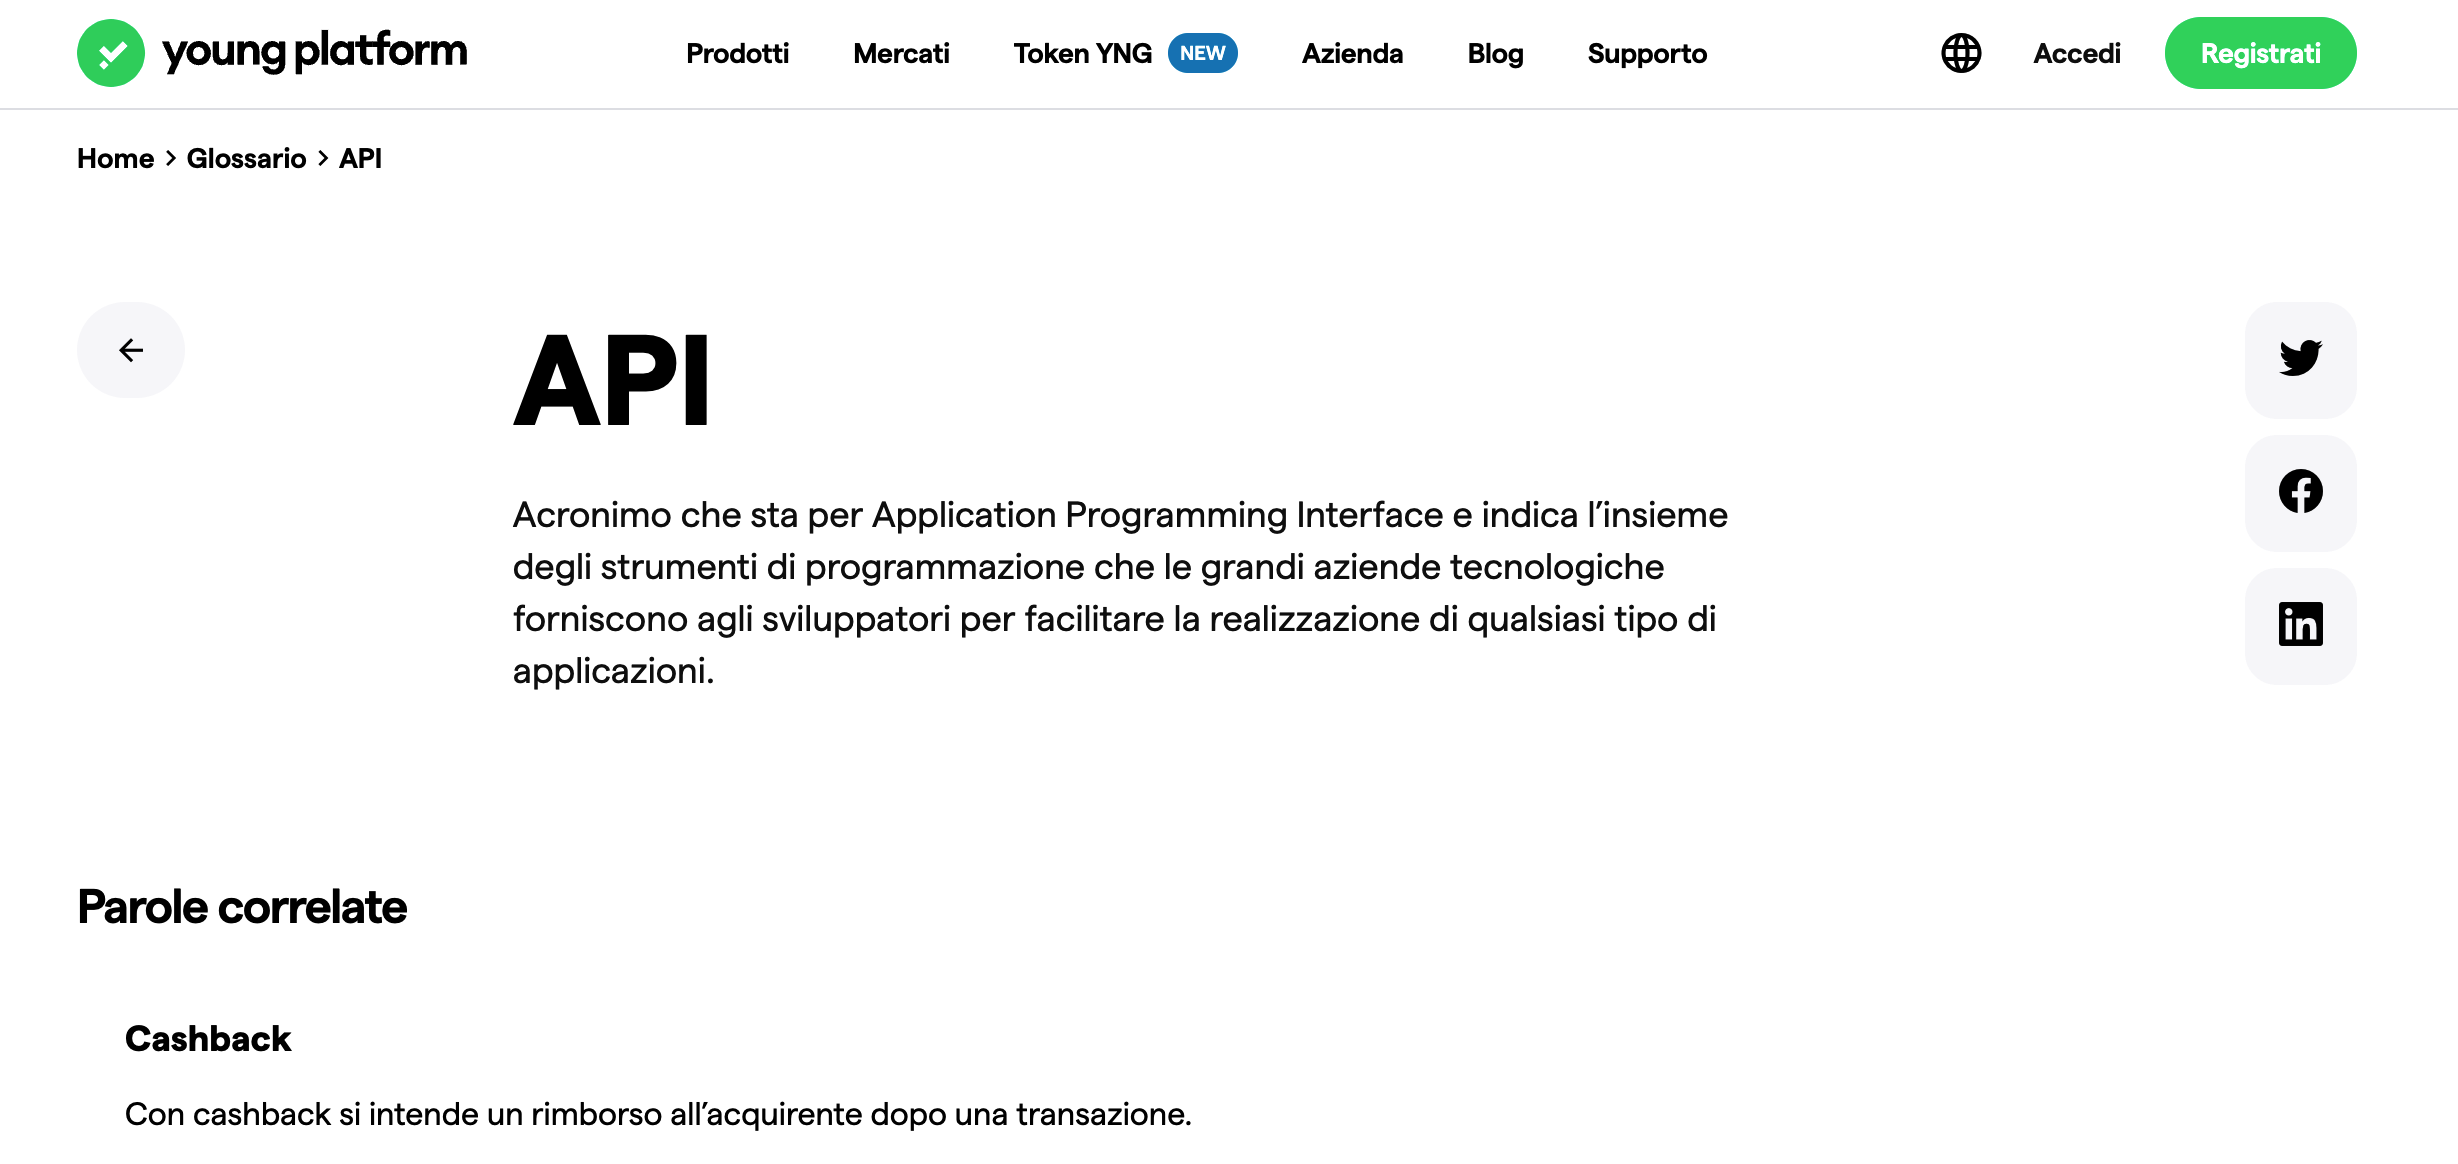
\includegraphics[width=0.80\textwidth]{res/images/internal-pages/glossary/glossary-4.png}
  \caption{Page that describes the meaning of the term \textit{API}.}
  \label{fig:glossary-4}
\end{figure}

\paragraph{Who}

The company logo is always present at the top left, as shown in the figure 
\ref{fig:glossary-4}.

\paragraph{Where}

Also on this page there is a \textit{breadcrumb} and it allows the user 
not to be confused. The use of this element allows to effectively 
communicate most of the where axis (top left, under the company logo, 
fig. \ref{fig:glossary-4}). There is another element on the page that 
increases the usability of the site: in the figure \ref{fig:academy-4} on 
the left there is an arrow that allows you to go back, that is, to the 
\textit{Glossario} (\textit{Glossary}) page. 

\paragraph{Why}

A novice user has more reasons than an experienced user to stay on this 
page, as a beginner has reached this page to inquire about very specific 
content. Furthermore, after the definition of the term searched, there is 
a section in which there is a list of terms closely related to the term 
searched (fig. \ref{fig:glossary-5}). This section is very important 
because the user can search for different terms and all of them follow a 
common thread starting from the term searched initially. 

\begin{figure}[H]
  \centering
  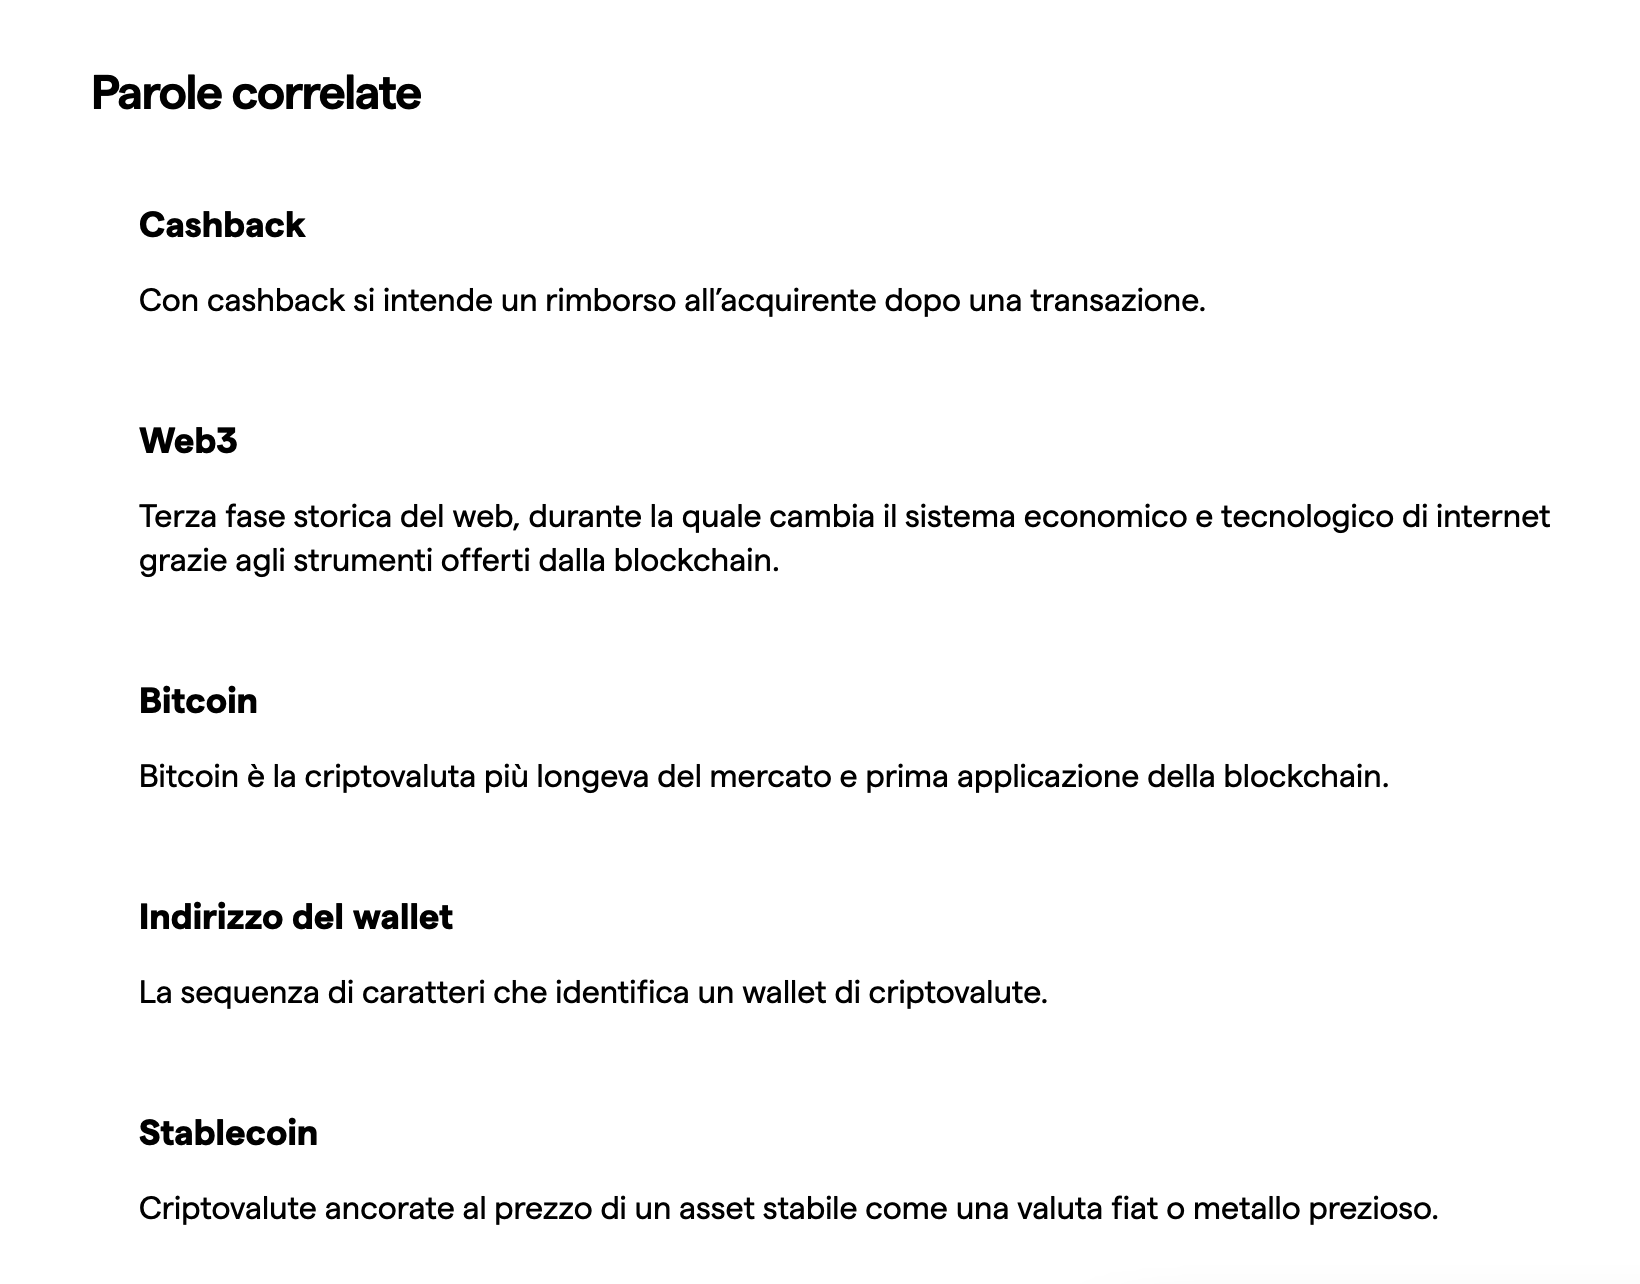
\includegraphics[width=0.80\textwidth]{res/images/internal-pages/glossary/glossary-5.png}
  \caption{Related terms starting with the term \textit{API}.}
  \label{fig:glossary-5}
\end{figure}

\paragraph{When}

There is no time reference on this page.

\paragraph{How}

This specific page is difficult to reach. However, access to this page is 
facilitated if you access to the \textit{Glossario} (\textit{Glossary}) 
page, as there are tools that facilitate reaching this page.

\subsubsection{Blog page}

The page can be reached at the following address: 
\href{https://youngplatform.com/blog/}{https://youngplatform.com/blog/}.

\paragraph{What}

The intentions of this page are explicit, that is, to provide a series of 
contents, so that users can stay up to date on all the latest news in this 
sector. In addition, the various articles are also cataloged, in order to 
understand the context they deal with.

\begin{figure}[H]
  \centering
  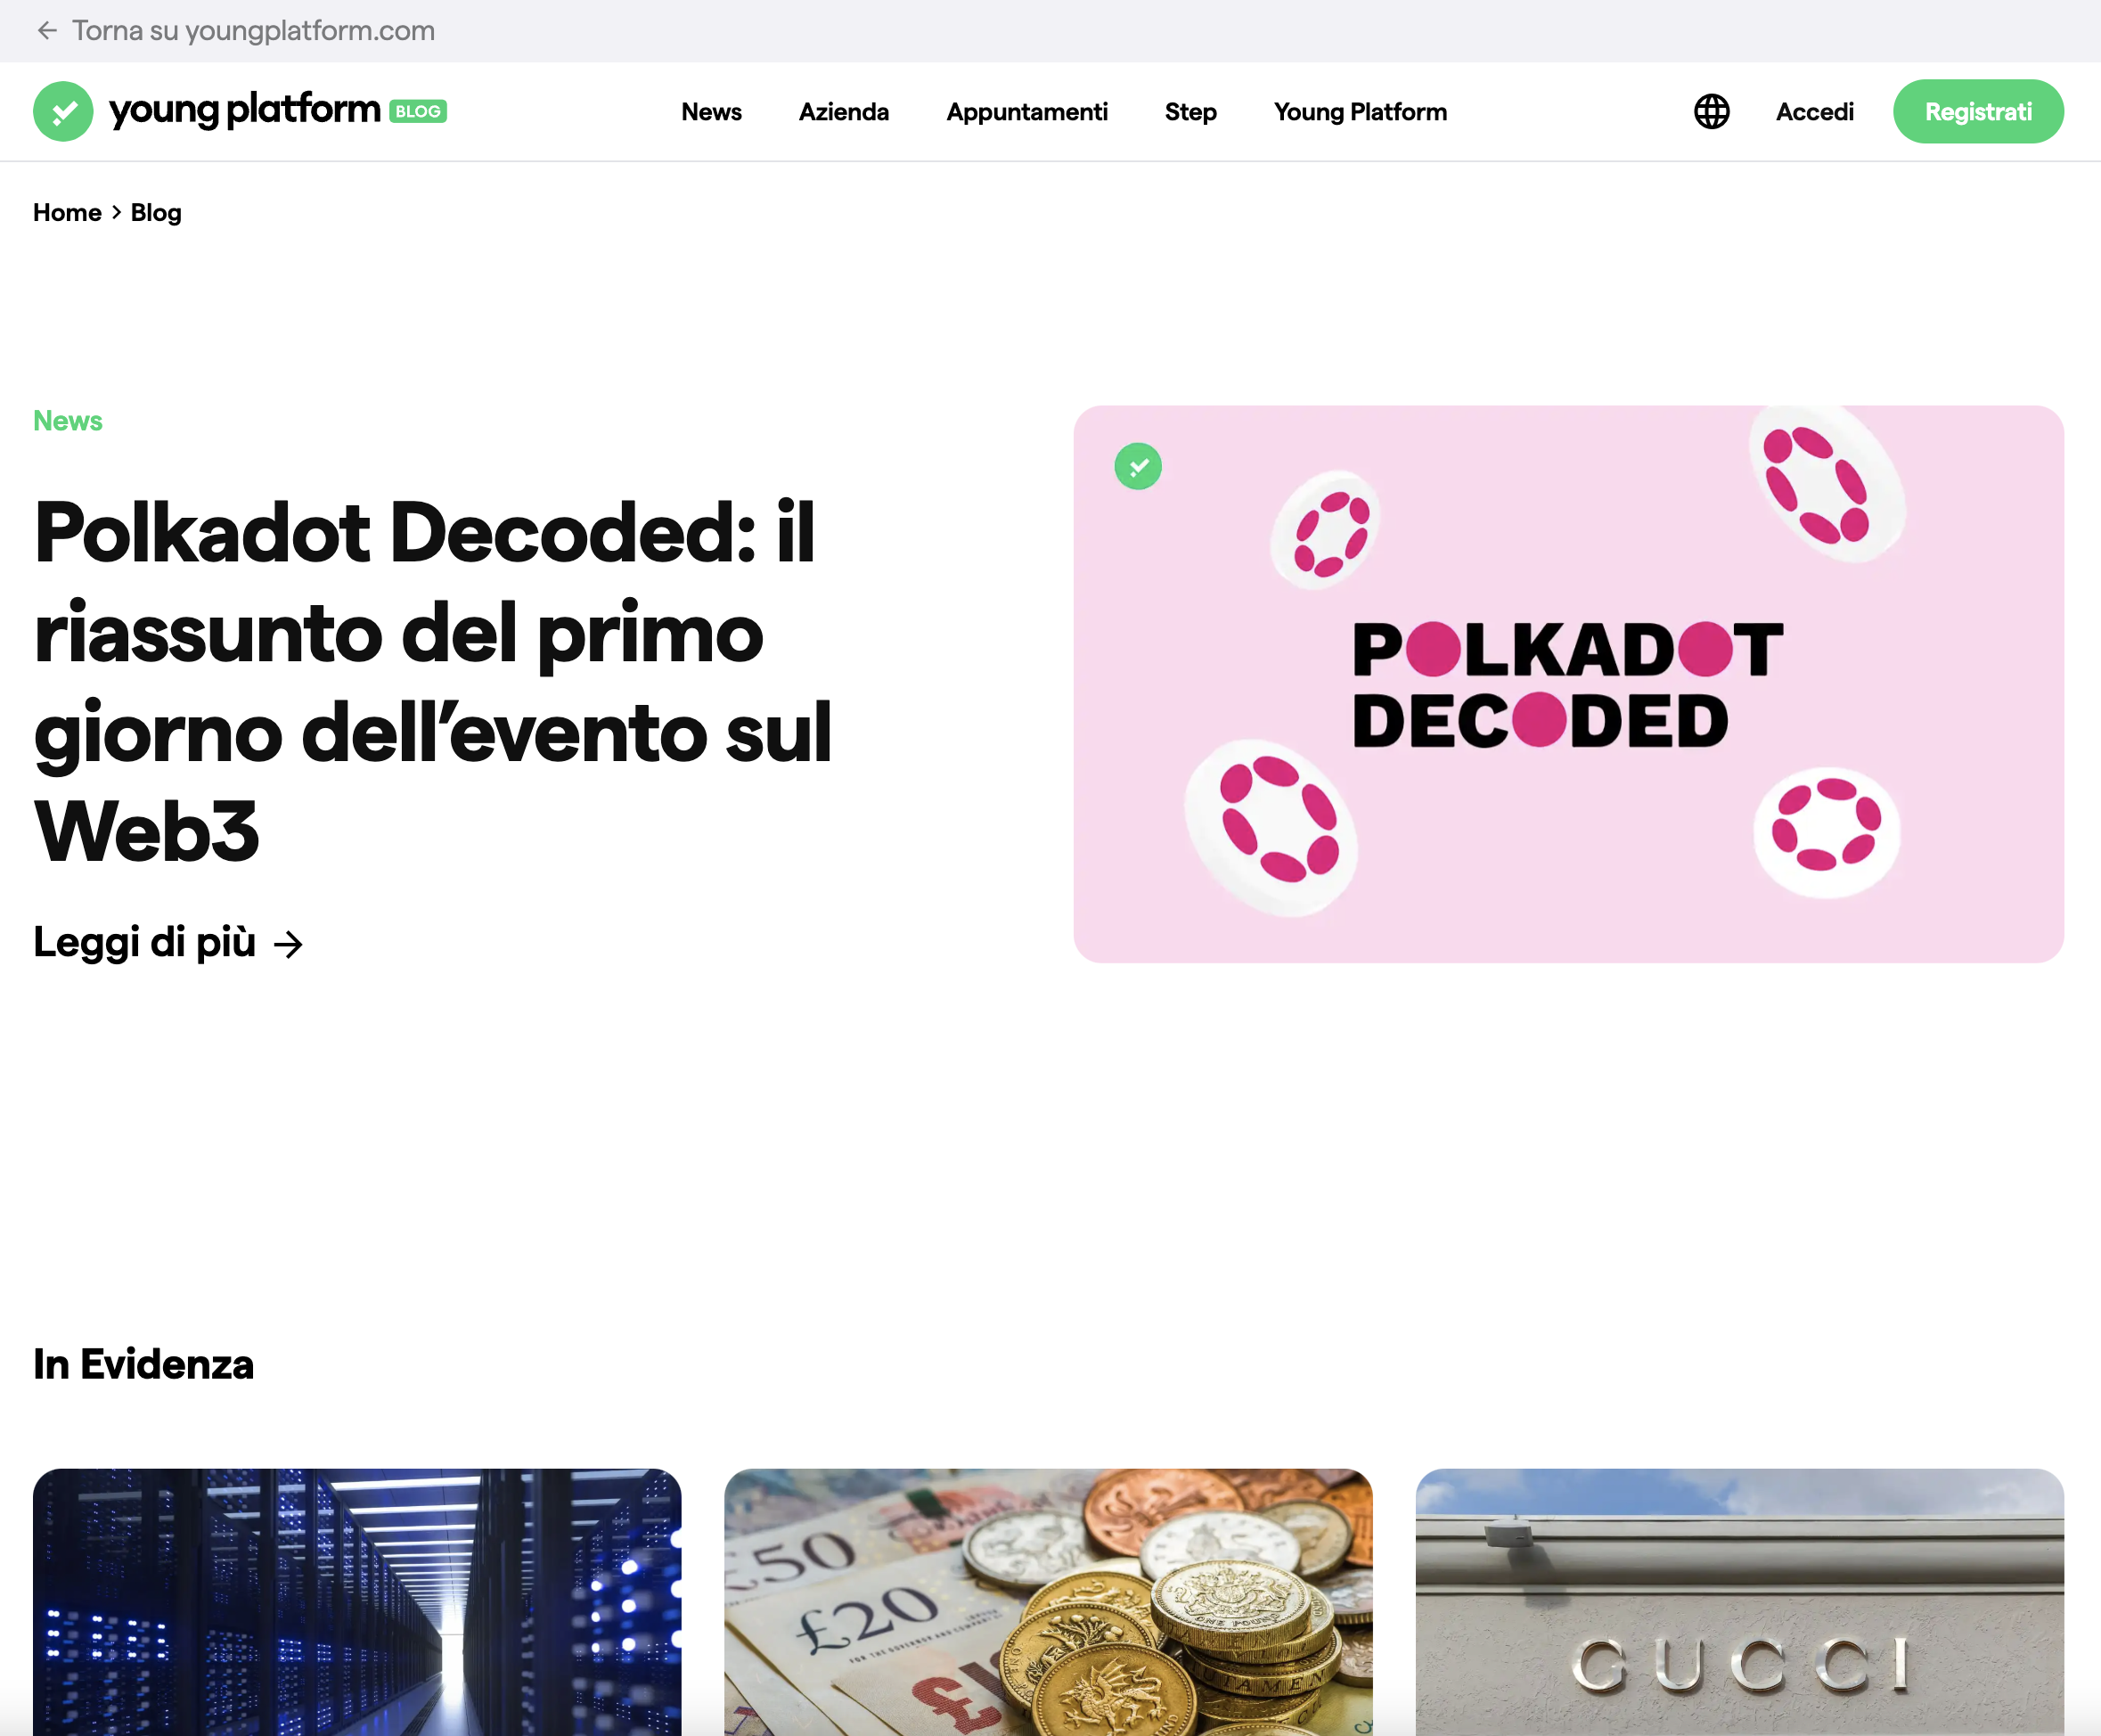
\includegraphics[width=0.70\textwidth]{res/images/internal-pages/blog/blog-1.png}
  \caption{Blog page.}
  \label{fig:blog-1}
\end{figure}

\paragraph{Who}

The company logo is always present at the top left, as illustrated
in the figure \ref{fig:blog-1}.

\paragraph{Where}

Also on this page there is a \textit{breadcrumb} and it allows the user 
not to be confused. The use of this element allows to effectively 
communicate most of the where axis (top left, under the company logo, 
fig. \ref{fig:blog-1}). There is another element on the page that 
increases the usability of the site: in the figure \ref{fig:blog-1}, above 
the company logo, there is an arrow and a text 
\textit{Torna su youngplatform.com} (\textit{Back to youngplatform.com}). 
This is a point of reference for returning directly to the homepage.

\paragraph{Why}

Regardless of the user's experience, the reasons to continue exploring 
this page are:
\begin{itemize}
  \item To stay up to date on the latest technological innovations;
  \item To stay up to date on the latest news on the market;
  \item To compare different technological approaches;
  \item To learn different concepts, especially for newbies.
\end{itemize}

\paragraph{When}

In this page there are clear time references: it is possible to note that 
the articles on the page have the publication dates (fig. 
\ref{fig:blog-2}). Also, as shown in figure \ref{fig:blog-1}, the last 
published article is inserted in the initial section of this page, in 
order to highlight it.

\paragraph{How}

This page can easily be reached via the main homepage menu (fifth item, 
fig. \ref{fig:homepage-1}). However, if a user wants to search for a 
particular article, this is not possible as there is no search tool. This 
represents a serious disadvantage. In order to find a particular article, 
the user should search for it through a search engine, specifying the 
site. Scrolling the page, you can see that the articles are cataloged and 
each category has a \textit{Vedi tutti} (\textit{See all}) item (top right, 
fig. \ref{fig:blog-2}), where you are redirected to a page which contains 
all the articles of that category. These categories are also reported at the 
top of the page, next to the company logo. This allows a user to already 
have an overview of the various categories and if a user already has in 
mind what type of article he is looking for, this facilitates the 
achievement of the article. However, the choice to change the items of the 
main menu with respect to those of the homepage could cause a sense of 
disorientation in the user.

\begin{figure}[H]
  \centering
  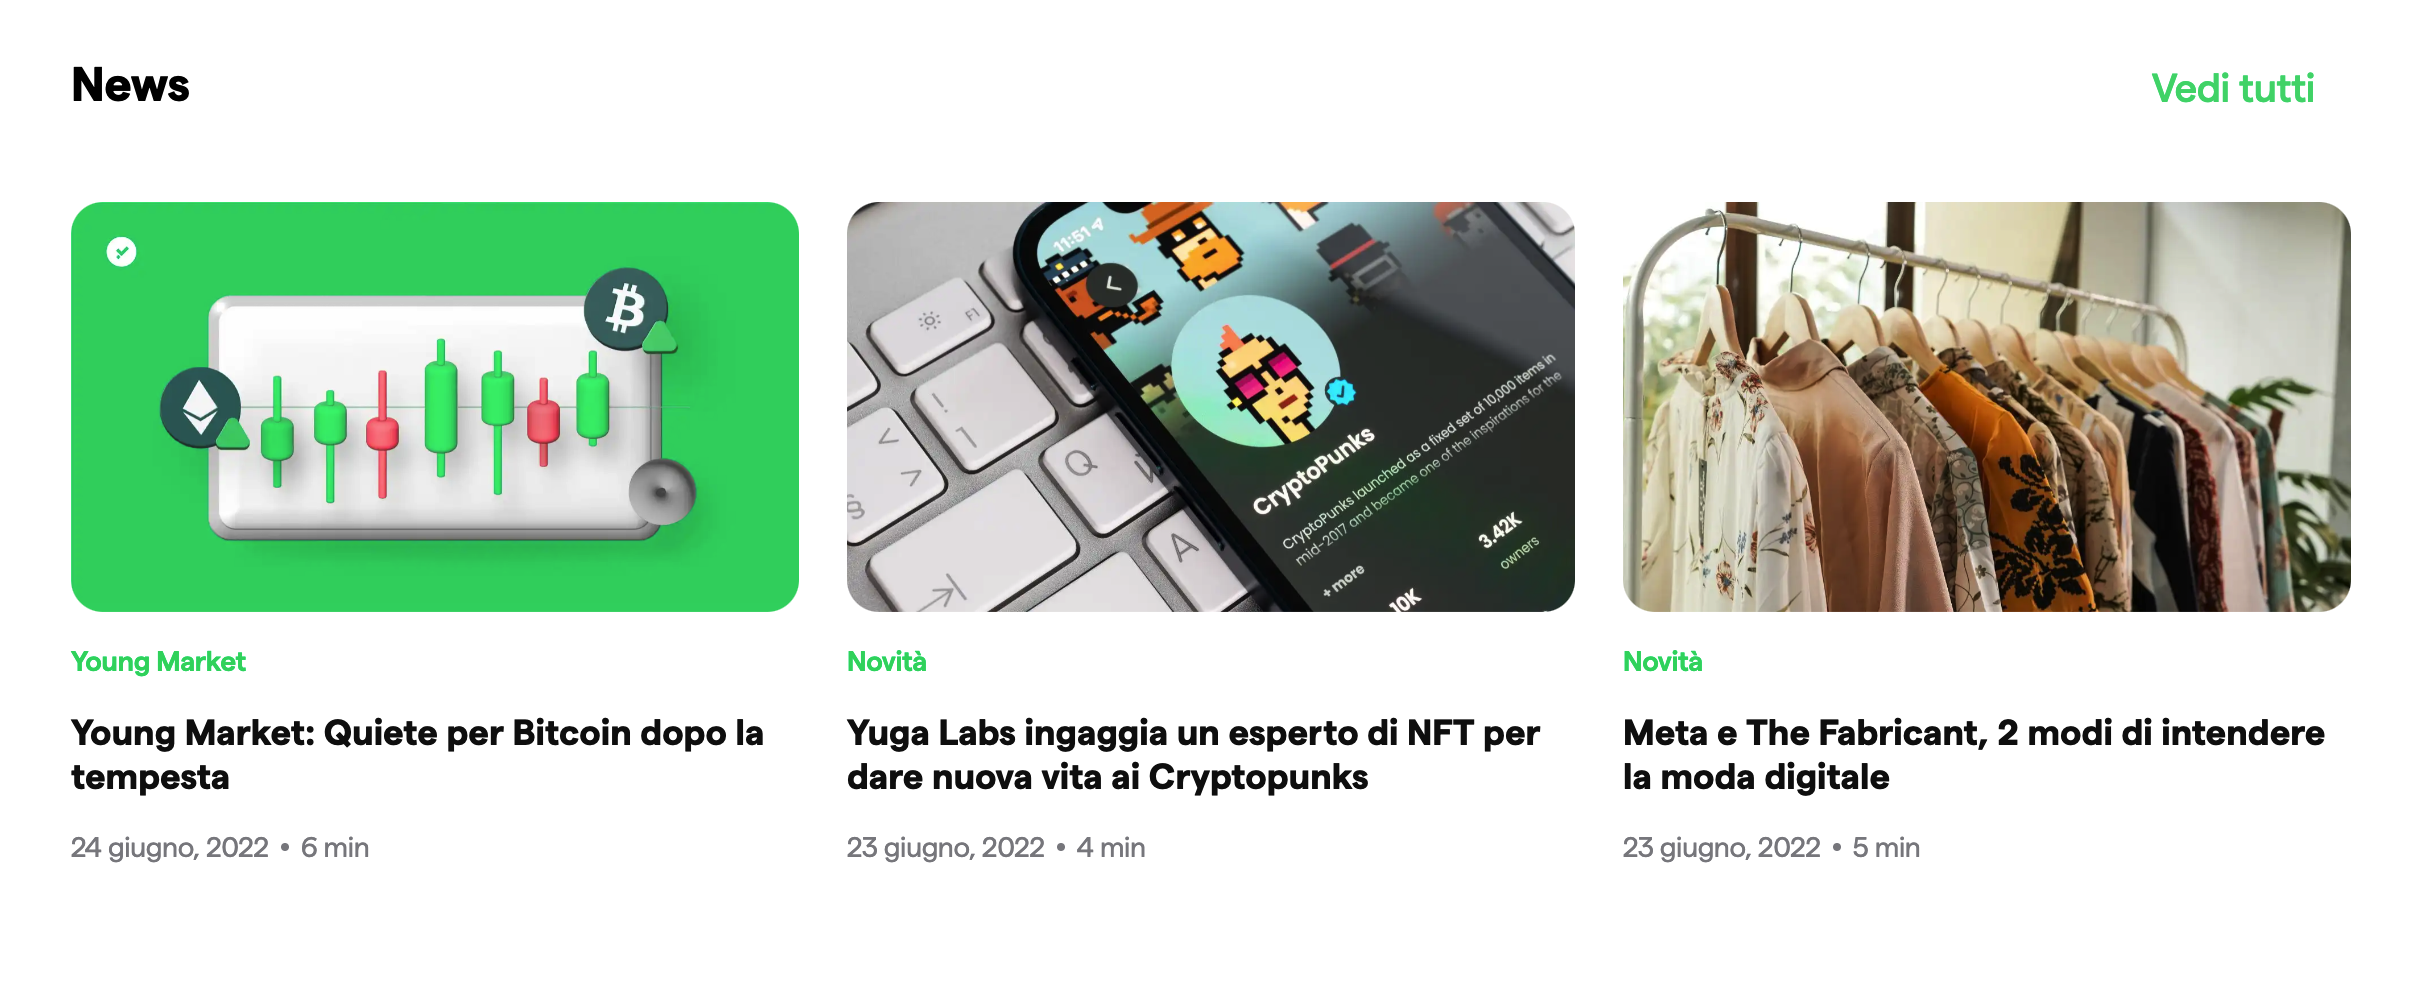
\includegraphics[width=0.80\textwidth]{res/images/internal-pages/blog/blog-2.png}
  \caption{One of the categories on the Blog page.}
  \label{fig:blog-2}
\end{figure}

\subsubsection{A blog article}

The page can be reached at the following address: \\
\href{https://youngplatform.com/blog/news/mercato-crypto-quiete-bitcoin-dopo-tempesta/}{https://youngplatform.com/blog/news/mercato-crypto-quiete-bitcoin-dopo-tempesta/}.

\paragraph{What}

The purpose of this specific page is clearly spelled out by the title. In 
fact, the title introduces what the content of the article will be.

\begin{figure}[H]
  \centering
  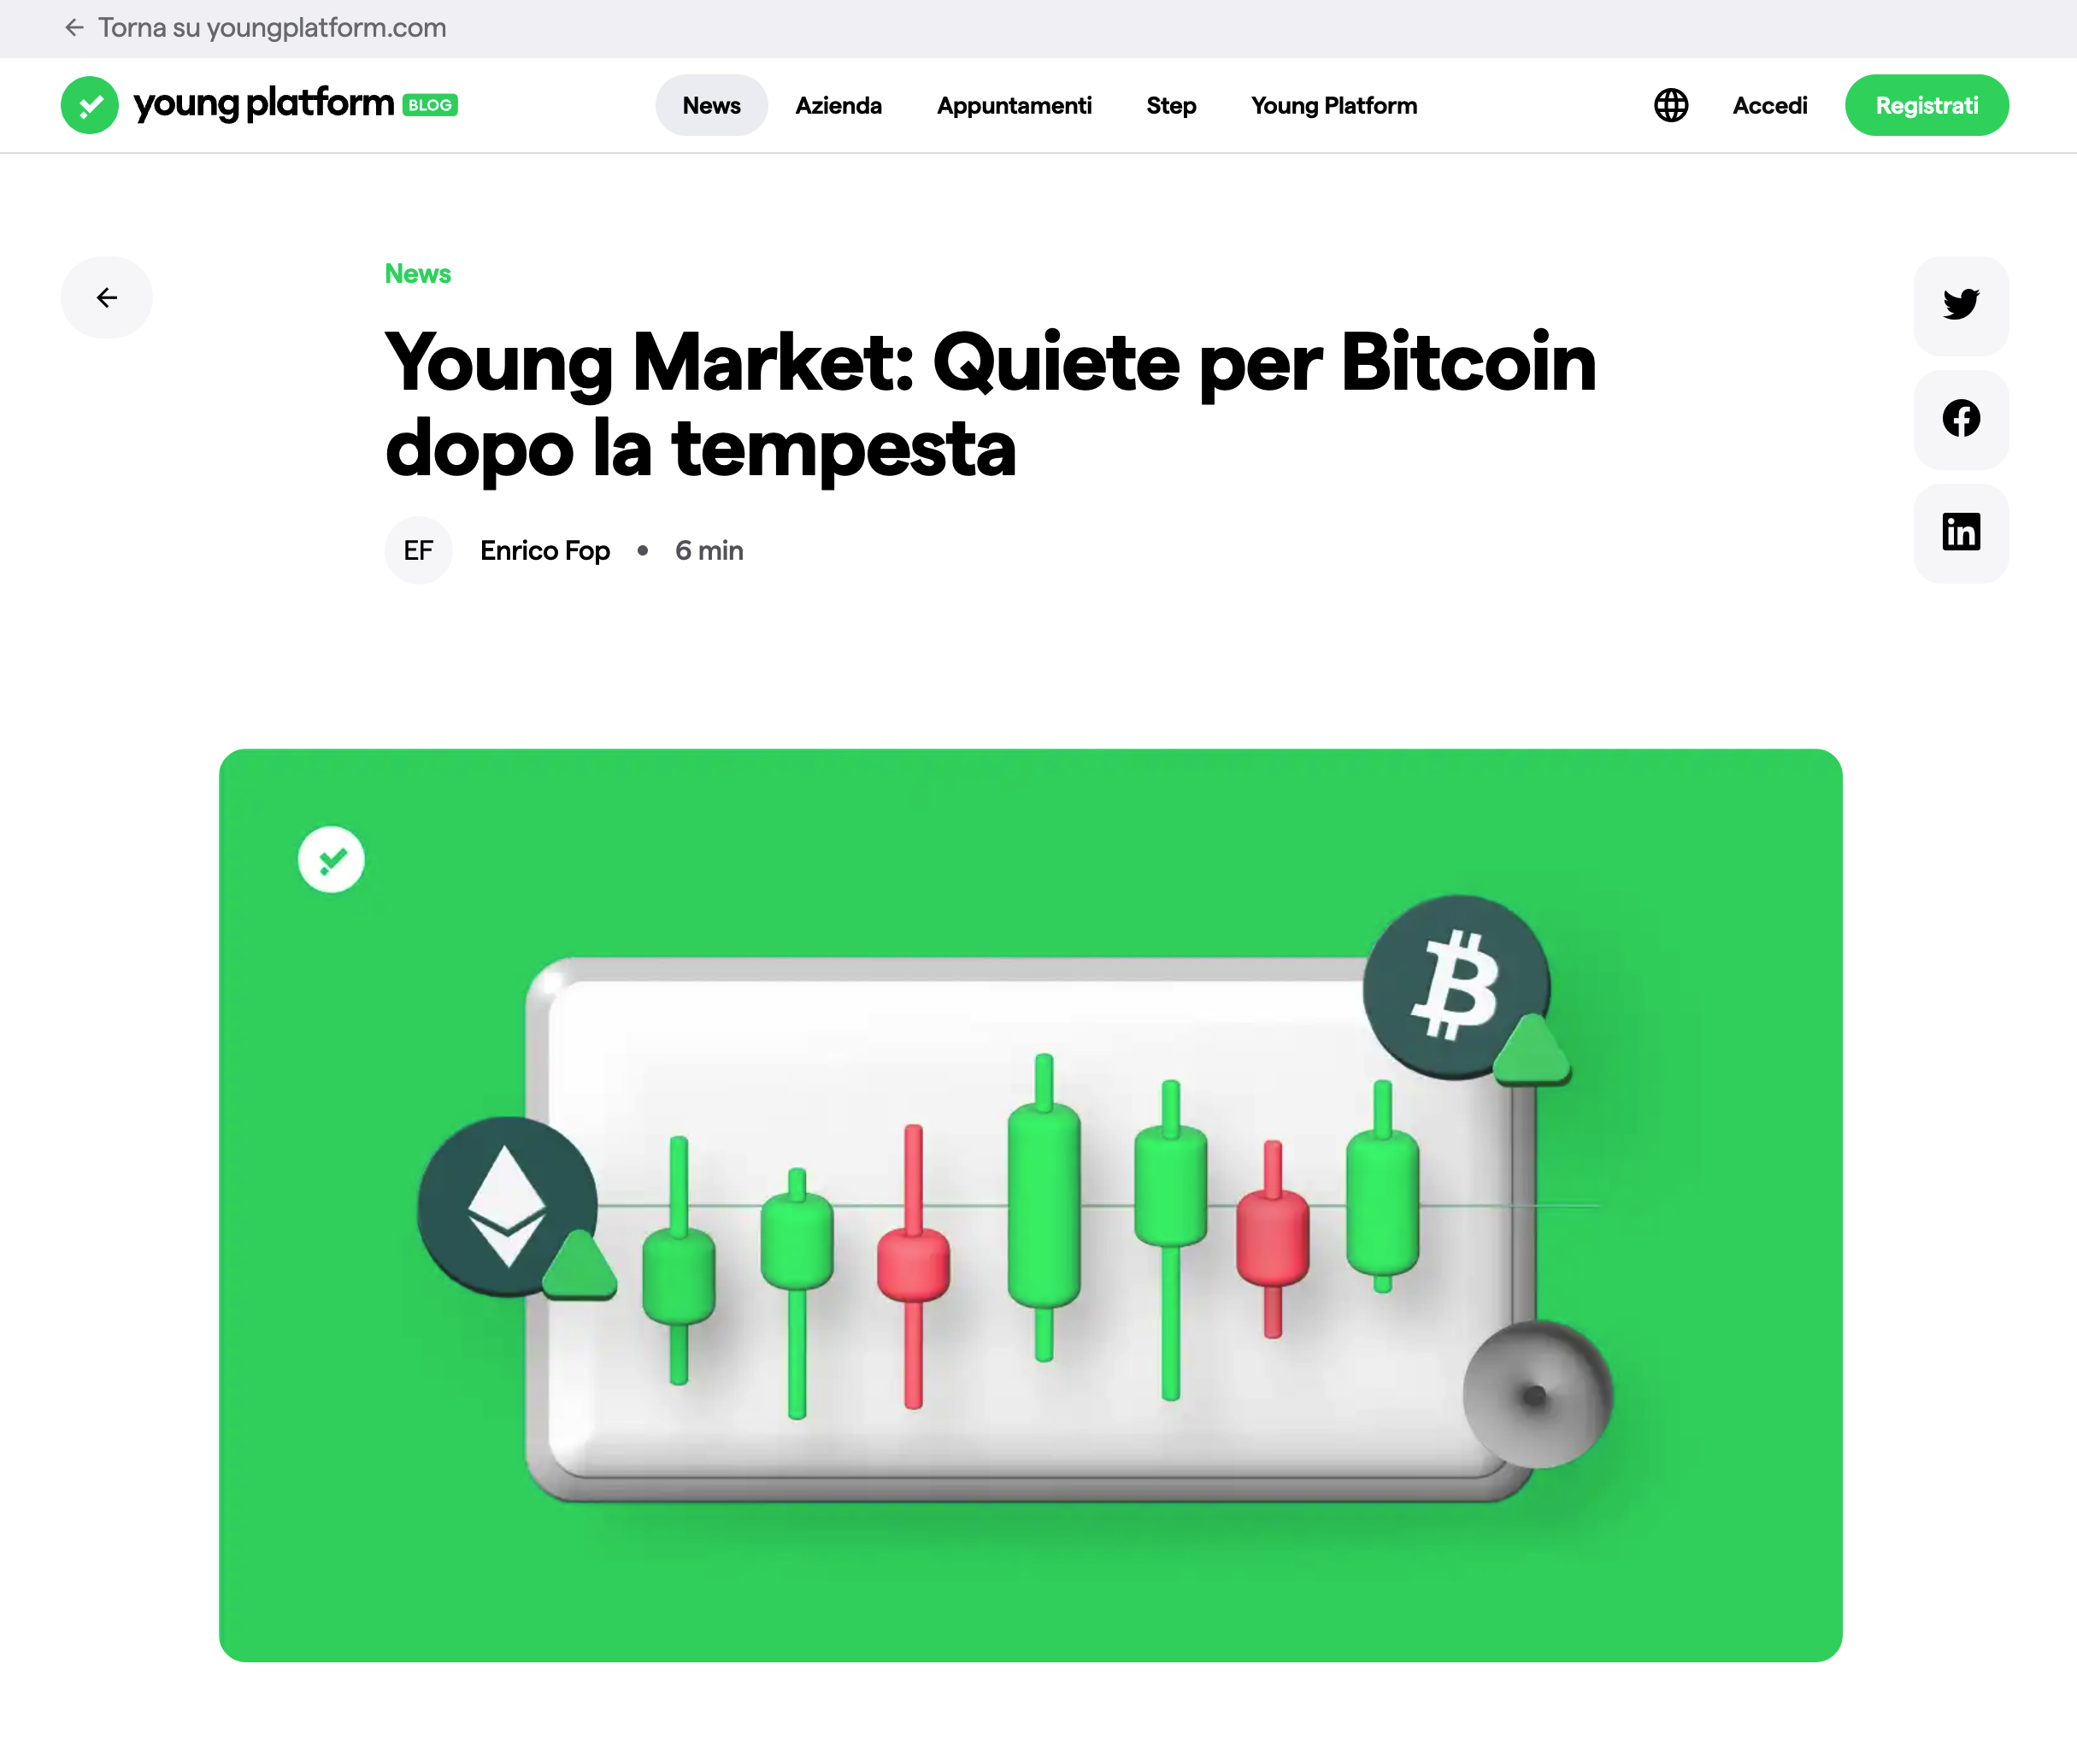
\includegraphics[width=0.80\textwidth]{res/images/internal-pages/blog/blog-3.png}
  \caption{A blog article.}
  \label{fig:blog-3}
\end{figure}

\paragraph{Who}

The company logo is always present at the top left, as shown in the figure 
\ref{fig:blog-3}.

\paragraph{Where}

There is an element on the page that increases the usability of the site: 
in figure \ref{fig:blog-3} on the left there is an arrow that allows you 
to go back, in the blog page. This element always remains in the same 
position even if the user scrolls the page. This is a positive aspect 
because if the user wants to return to the previous page, it is not 
necessary for the user to return to the top of the page. Furthermore, 
in the figure \ref{fig:blog-3}, above the company logo, there is an 
arrow and a text \textit{Torna su youngplatform.com} (\textit{Back to 
youngplatform.com}). This is a point of reference for returning directly 
to the homepage. Compared to the articles of the \textit{Academy}, there 
is no bar showing how far the user has reached to read the article.

\paragraph{Why}

The main reason for continuing to explore the page is because the user 
(whether novice or expert) is interested in reading this specific article. 
Furthermore, at the end of the page there is a section that invites you to 
read other articles related to the one you have just read.

\paragraph{When}

Although in the \textit{Blog} page there are clear time references, in the 
specific page of the article there is no date of publication of the article.

\paragraph{How}

Reaching this specific page is difficult. It can be reached by browsing the 
\textit{Blog} page or by using a search engine. This represents a major 
disadvantage for the user, as the user would have to spend a lot of time 
browsing the blog before finding the article, or would have to leave the 
site to access a search engine.

\subsubsection{Support page}

The page can be reached at the following address: 
\href{https://support.youngplatform.com/hc/it}{https://support.youngplatform.com/hc/it}.

\begin{figure}[H]
  \centering
  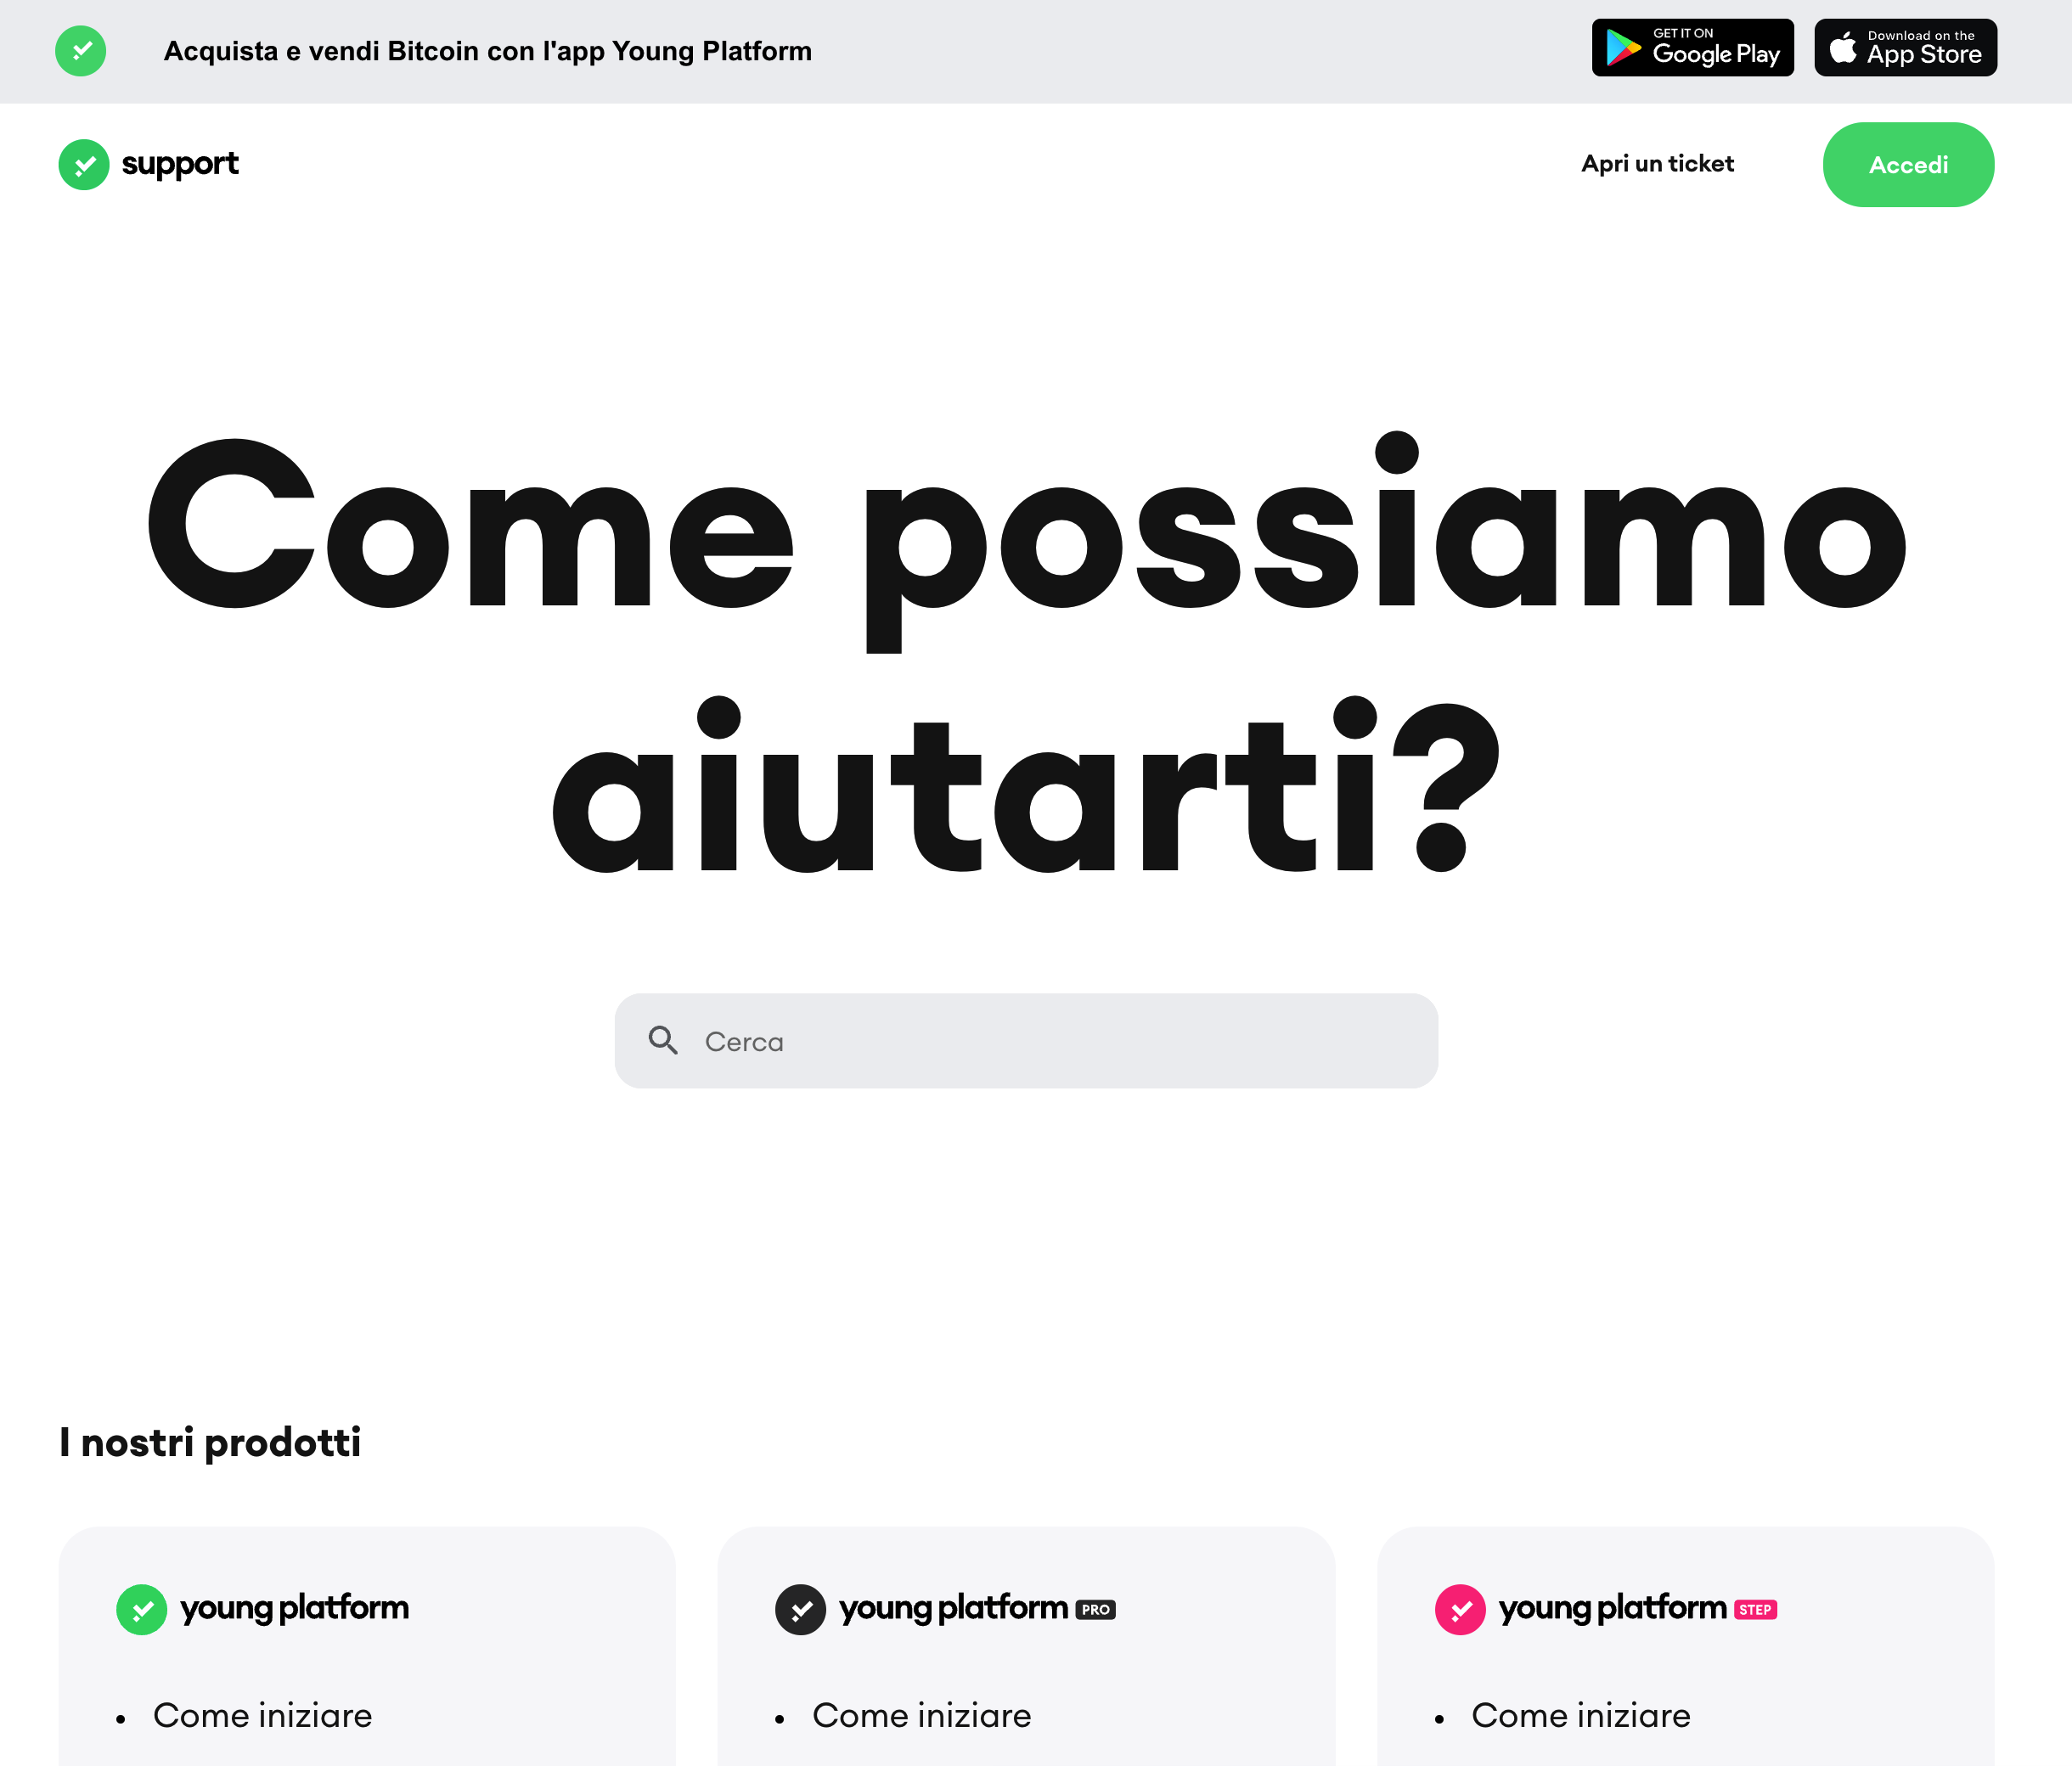
\includegraphics[width=0.70\textwidth]{res/images/internal-pages/support/support-1.png}
  \caption{First section of the \textit{Support} page.}
  \label{fig:support-1}
\end{figure}

\paragraph{What}

The goal of this page is immediately clear. The purpose of this page is to 
provide support and help to the user. The page allows you to offer 
different "types" of support:
\begin{itemize}
  \item \textit{Search bar}: the user can enter terms related to his 
  problem and obtain related results (fig. \ref{fig:support-2});

  \begin{figure}[H]
    \centering
    
\includegraphics[width=0.60\textwidth]{res/images/internal-pages/support/support-2.png}
    \caption{Search tool.}
    \label{fig:support-2}
  \end{figure}
  
  \item \textit{FAQ divided by product} (fig. \ref{fig:support-3});
  
  \begin{figure}[H]
    \centering
    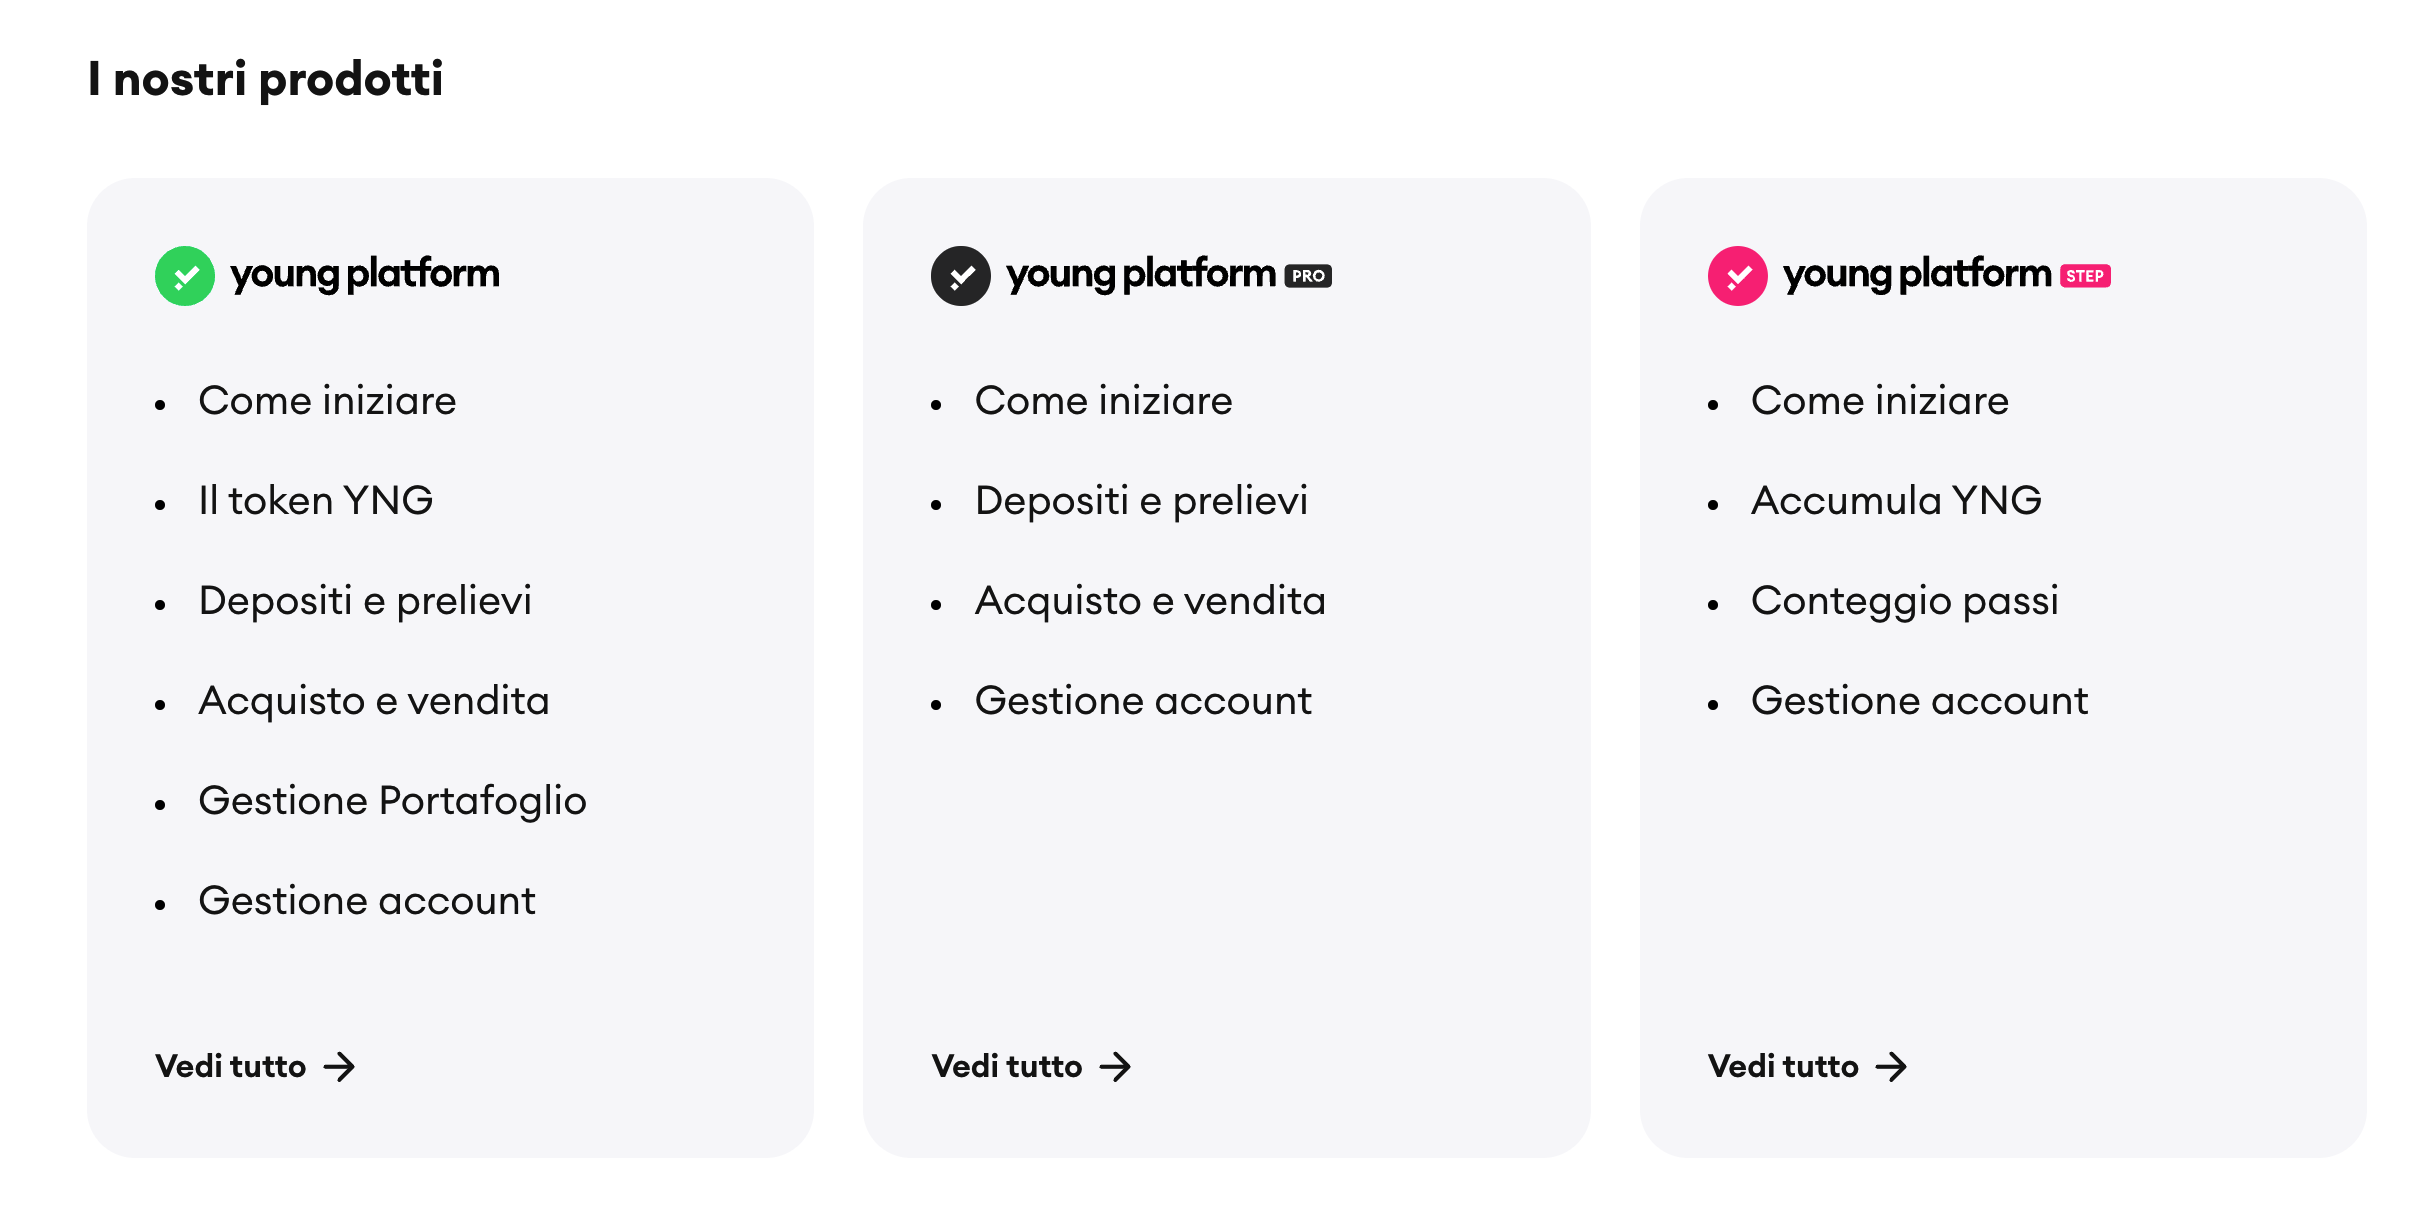
\includegraphics[width=0.80\textwidth]{res/images/internal-pages/support/support-3.png}
    \caption{Some FAQs divided by product.}
    \label{fig:support-3}
  \end{figure}
  
  \item \textit{Blog articles} (fig. \ref{fig:support-4});
  
  \item \textit{Articles from the Academy} (fig. \ref{fig:support-5});
  
  \item \textit{Link to social networks and to the newsletter} 
  (fig. \ref{fig:support-6}).
\end{itemize}

\begin{figure}[H]
  \centering
  
\includegraphics[width=0.60\textwidth]{res/images/internal-pages/support/support-4.png}
  \caption{Section that redirects to the \textit{Blog}.}
  \label{fig:support-4}
\end{figure}

\begin{figure}[H]
  \centering
  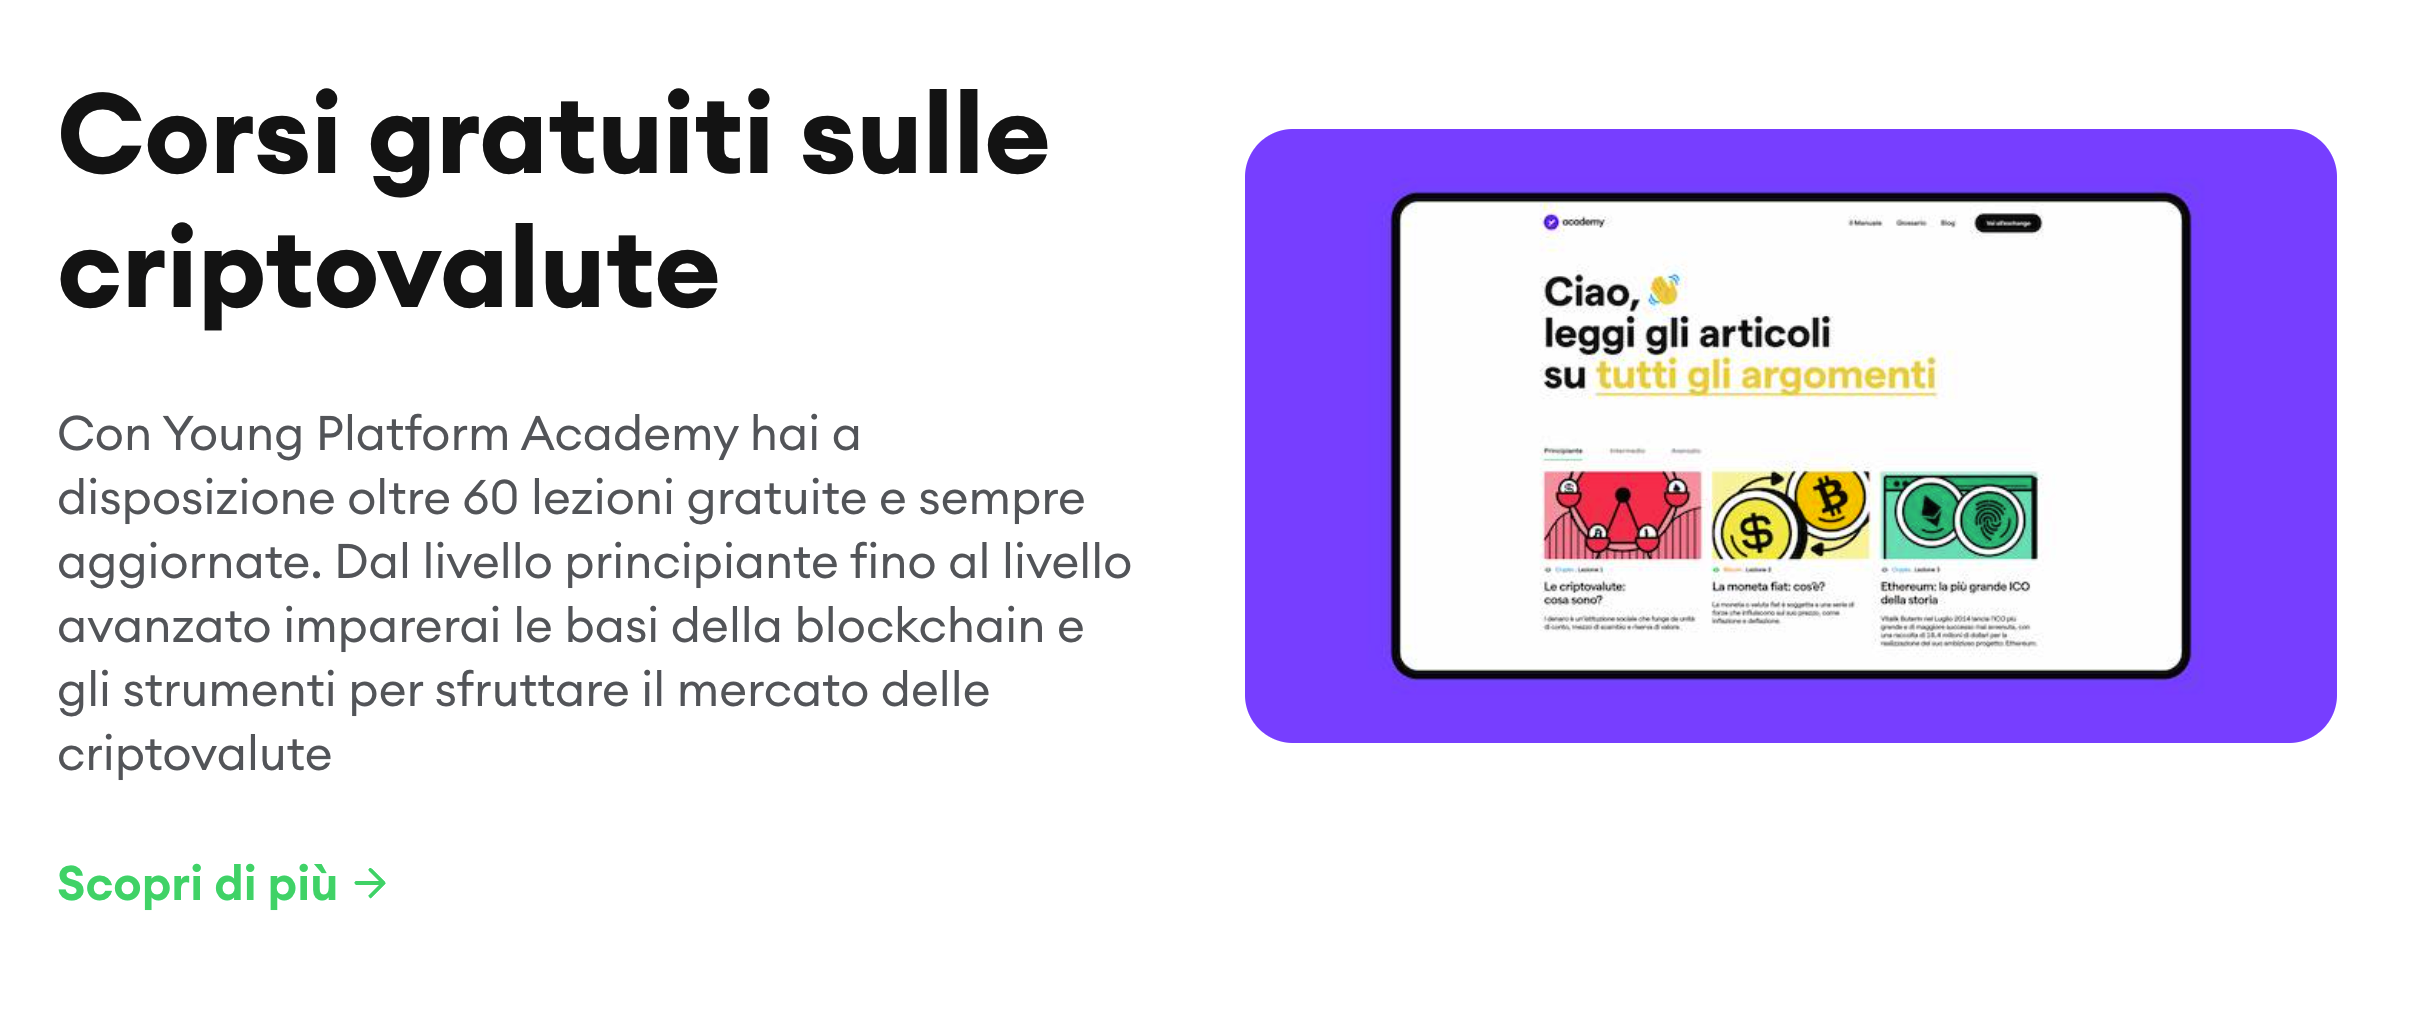
\includegraphics[width=0.80\textwidth]{res/images/internal-pages/support/support-5.png}
  \caption{Section that redirects to the \textit{Academy}.}
  \label{fig:support-5}
\end{figure}

\begin{figure}[H]
  \centering
  
\includegraphics[width=0.80\textwidth]{res/images/internal-pages/support/support-6.png}
  \caption{Elements that allow the user to stay in touch with the 
  community (social networks and newsletters).}
  \label{fig:support-6}
\end{figure}

The last type of support offered by the site is the possibility for the 
user to open \textit{ticket} for assistance. To do this, there is a 
button \textit{Apri un ticket} (\textit{Open a ticket}), located at the 
top right, to the left of the green button \textit{Accedi} (\textit{Login}), 
as shown in the figure \ref{fig:support-1}. 

\paragraph{Who}

The company logo is always present at the top left, as shown in the figure 
\ref{fig:support-1}.

\paragraph{Where}

When the user is redirected to this page, they may notice that they have 
arrived at a new subdomain (\textit{support.youngplatform.com}). However, 
there is no element that allows you to return to the page you have reached 
or to return to the \textit{youngplatform.com} homepage. In order to return 
to the homepage, you need to go to the footer. This implementation is very 
disadvantageous for the user and requires some effort to perform the action.

\paragraph{Why}

Regardless of the user's experience, this page is of fundamental 
importance, as it allows to put the user in contact with company 
staff. So, the user first wants to explore this page to see if there are 
already any illustrated solutions. To explore the solutions already 
proposed by the site, the user can visit the various solutions divided 
by product (fig. \ref{fig:support-2}), or use the search bar (fig. 
\ref{fig:support-3}). Also, if the user does not find the answer to their 
problem, they can open a new ticket.

\paragraph{When}

There is no time reference on this page.

\paragraph{How}

This page is easy to reach from the homepage. It can be reached via the 
main homepage menu (fig. \ref{fig:homepage-1}) or via the footer (first 
item in the fourth column, fig. \ref{fig:footer}). In this page there are 
dedicated sections for the exploration of the articles of the \textit{Blog} 
(fig. \ref{fig:support-4}), for the exploration of the articles of the 
\textit{Academy} (fig. \ref{fig:support-5}) and to reach the various 
social networks (fig. \ref{fig:support-6}). Furthermore, the user can 
explore the solutions to different problems for each product through a 
special section, illustrated in figure \ref{fig:support-3}. If the user 
does not find the answer to their problem, then the site offers the 
possibility to send a \textit{ticket} to support. To do this, there is a 
\textit{Apri un ticket} (\textit{Open a ticket}) button, located at the 
top right, to the left of the green \textit{Accedi} (\textit{Login}) 
button (fig. \ref{fig:support-1}). I believe that, given the importance 
of this functionality, the element that allows to open a new ticket is 
located in the wrong place. At first glance, this element is not 
immediately recognizable and therefore the user may find himself 
disoriented (especially if the user is a beginner). I would have placed 
this element in a position that would have made it more visible, so 
that, even if the user does not need it, it is clearly visible at first 
sight. 